\chapter{Beispiel}
Dieses Kapitel bietet einen umfassenden Überblick über die Funktionalität und Benutzerfreundlichkeit der Anwendung. Anhand einer Reihe detaillierter Screenshots wird die Bedienung des Systems anschaulich dargestellt und analysiert. Dadurch erhalten die Leserinnen und Leser einen praxisnahen Einblick in den Umgang mit der Anwendung sowie die einzelnen Arbeitsschritte.

\section{Startseite}\index{Startseite}

Die Startseite der Anwendung dient als zentraler Einstiegspunkt für alle Nutzergruppen. Sie bietet einen Überblick über die wichtigsten Funktionen der App, wie die Buchsuche, aktuelle Empfehlungen und den Zugang zu weiterführenden Diensten. Die Benutzeroberfläche ist übersichtlich gestaltet und ermöglicht eine intuitive Navigation durch die verschiedenen Inhalte. In diesem Teil wird gezeigt, wie die Startseite strukturiert ist und welche interaktiven Elemente den Nutzerinnen und Nutzern zur Verfügung stehen.

\subsection{Header und Navigation}\index{Header und Navigation}
Die folgende Abbildung \ref{fig:header} zeigt den Aufbau des Headers mit dem dynamischen Navigationsmenü, das sich je nach Benutzerrolle unterscheidet:

\begin{figure}[H]
	\centering
	
\includegraphics[width=1.0\textwidth]{images/UI-screenshots/Header.png}
	\caption{ Kopfzeile der App \textit{Libranova}}
	\label{fig:header}
\end{figure}

\begin{itemize}
	\item \textbf{Besucher:} Anzeige des \textit{Libranova}-Logos sowie der Menüpunkte \textbf{Startseite} und \textbf{Bücher Suchen}. Rechts oben befindet sich ein \textbf{Login}-Button. Außerdem steht ein Dropdown-Menü zur Auswahl der Sprache (Deutsch oder Englisch) zur Verfügung.
	\item \textbf{Eingeloggte Nutzer:} Zusätzlich zu den Besucher-Menüpunkten sind \textbf{Bibliotheksaktivität} (Einblick in ausgeliehene Bücher und Ausleihhistorie) sowie \textbf{Überfällige Gebühren} (Anzeige möglicher Gebühren für verspätete Rückgaben) sichtbar. Rechts oben wird ein \textbf{Logout}-Button angezeigt. 
	\item \textbf{Administratoren:} Alle Menüpunkte der eingeloggten Nutzer plus der Menüpunkt \textbf{Admin}, welcher Verwaltungsfunktionen für den Buchbestand (Hinzufügen, Ändern, Löschen) und die Bearbeitung von Kundenanfragen umfasst.
\end{itemize}

\subsection{Footer}\index{Footer}
Die folgende Abbildung \ref{fig:footer} zeigt die Fußzeile der Anwendung. Sie enthält das Copyright \textcopyright\ Libranova App, Inc sowie die Menüpunkte \textbf{Startseite} und \textbf{Bücher suchen}.

\begin{figure}[H]
	\centering
	
\includegraphics[width=1.0\textwidth]{images/UI-screenshots/Footer.png}%\subsection{Startseite (Main Page)}
	\caption{ Kopfzeile der App \textit{Libranova}}
	\label{fig:footer}%\subsubsection{Karussell (Carousel)}
\end{figure}

\subsection{Hauptteil}\index{Hauptteil}

\subsection*{Karussell und Buch-Browser}\index{Karussell und Buch-Browser}

Die folgende Abbildung  \ref{fig:Carousel_and_BookBrowser} zeigt ein Karussell zur Darstellung ausgewählter Bücher sowie einen Button, der zur Suchseite für Bücher weiterleitet.

\begin{figure}[H]
	\centering
	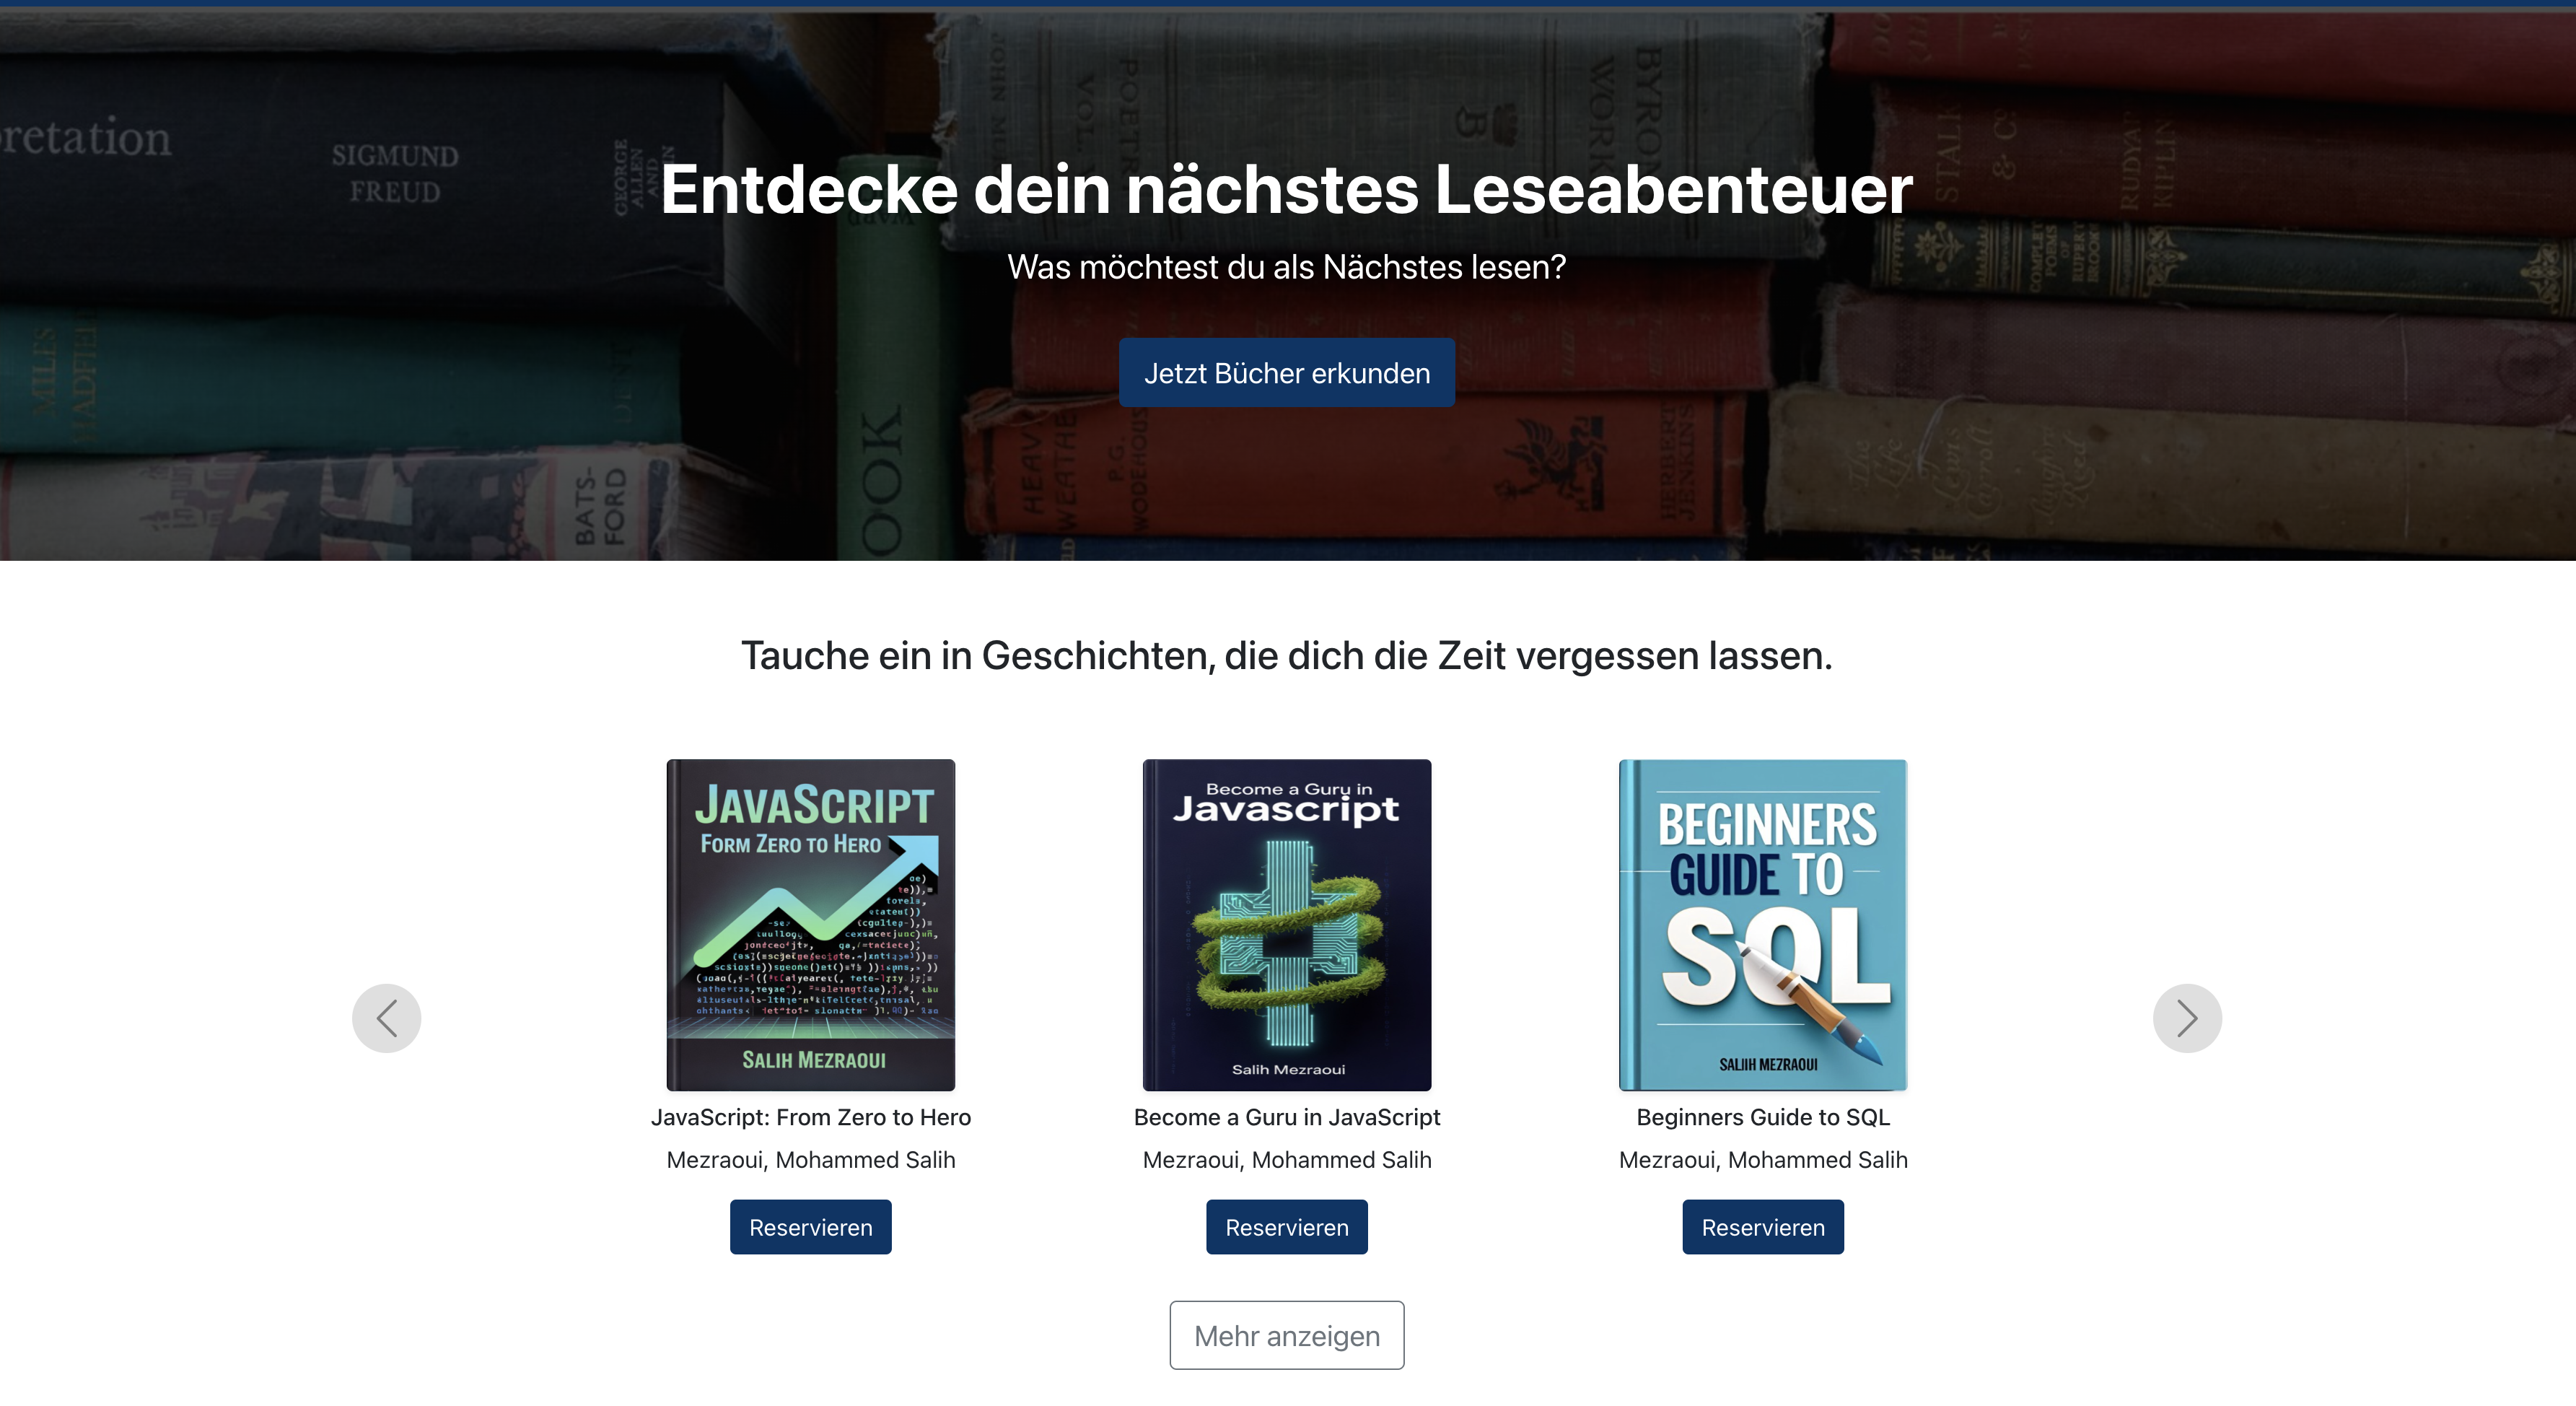
\includegraphics[width=1.0\textwidth]{images/UI-screenshots/Carousel_and_BookBrowser.png}%\subsection{Startseite (Main Page)}
	\caption{Karussell und Buch-Browser-Schaltfläche}
	\label{fig:Carousel_and_BookBrowser}%\subsubsection{Karussell (Carousel)}
\end{figure}

\subsection*{}\index{Link zur Bibliotheksdienste}

Die folgende Abbildung \ref{fig:Bibliotheksdienste-Link} zeigt einen Link zu den Bibliotheksdiensten, der angezeigt wird, wenn der Benutzer angemeldet ist. Andernfalls erscheint die Option ‚Registrieren‘.

\begin{figure}[H]
	\centering
	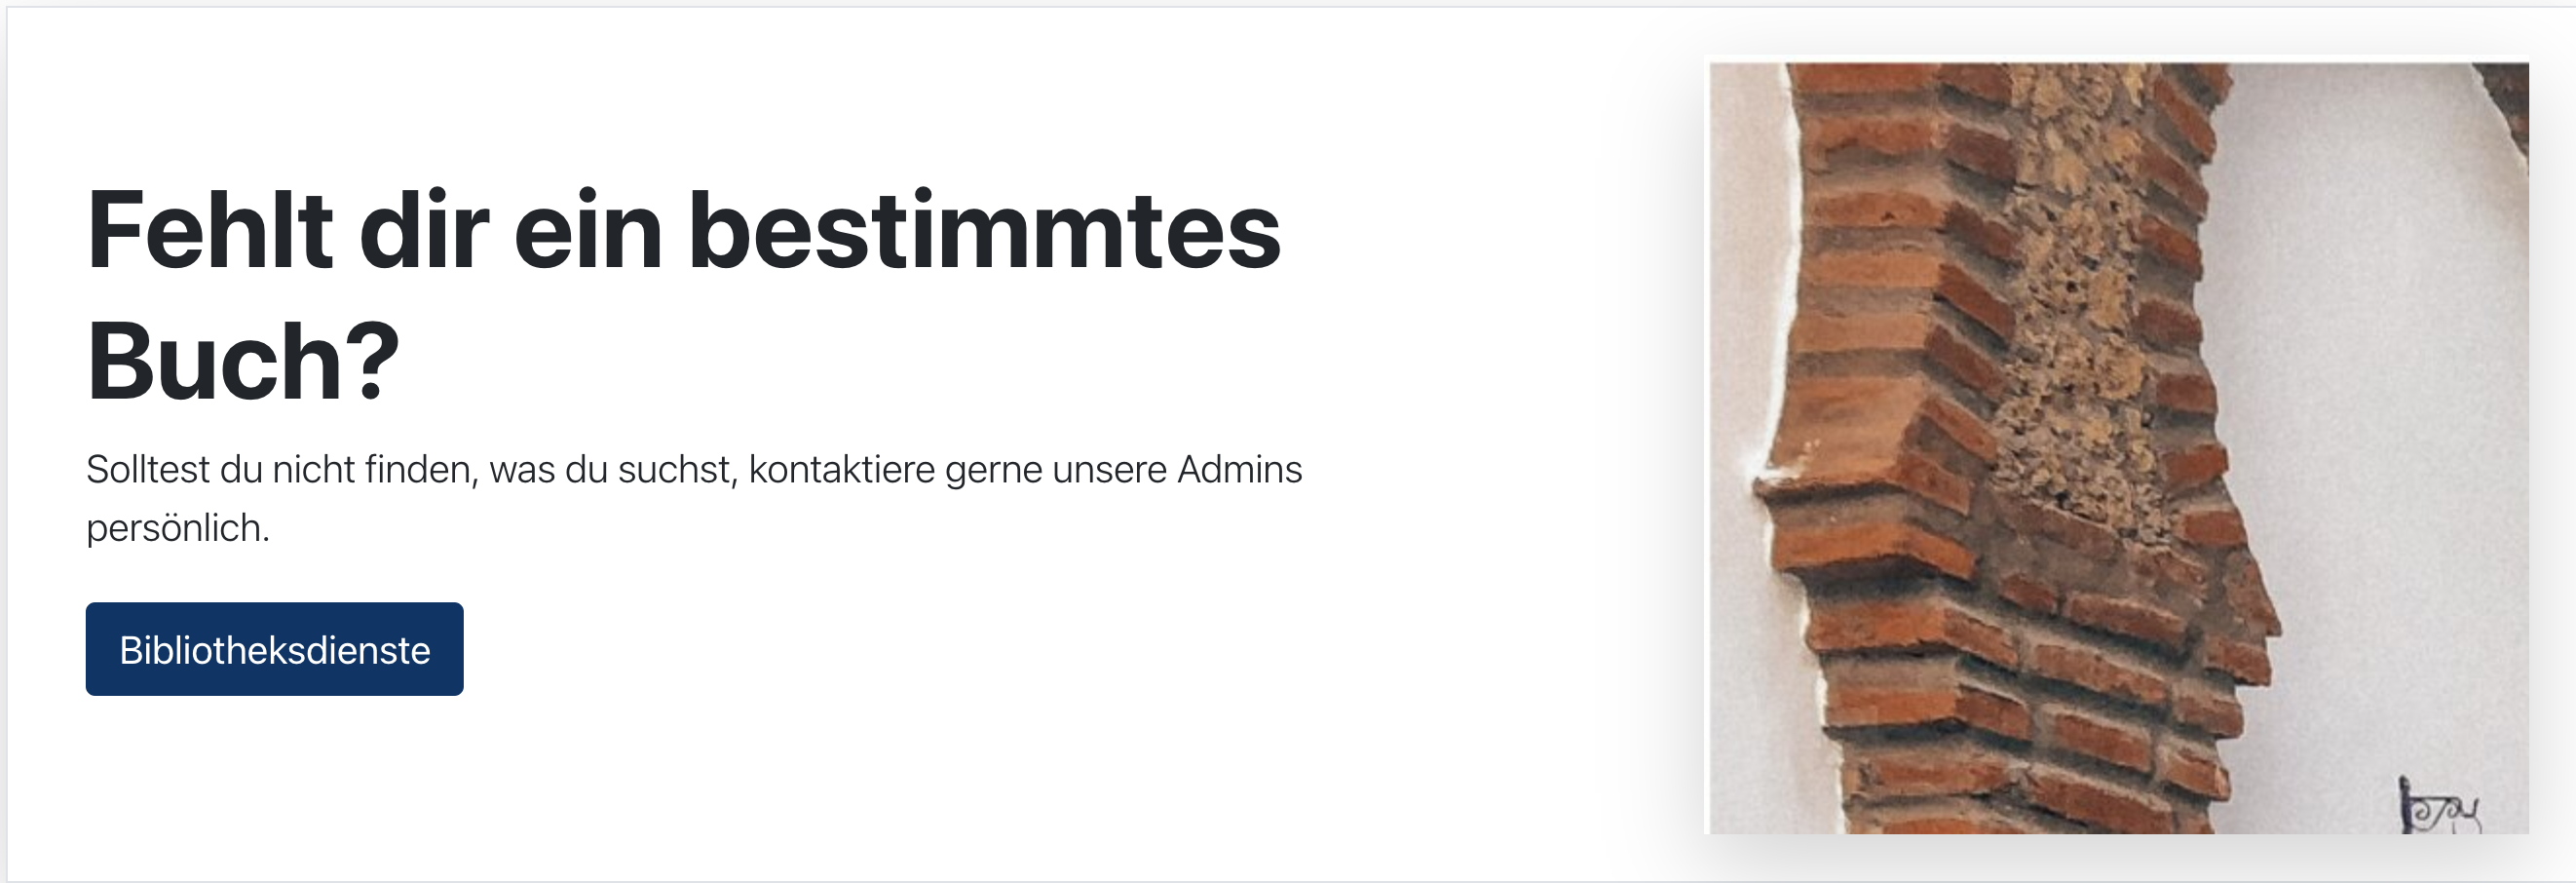
\includegraphics[width=1.0\textwidth]{images/UI-screenshots/Bibliotheksdienste-Link.png}%\subsection{Startseite (Main Page)}
	\caption{Karussell und Buch-Browser-Schaltfläche}
	\label{fig:Bibliotheksdienste-Link}%\subsubsection{Karussell (Carousel)}
\end{figure}

\section{Seitenübersicht}
Dieser Abschnitt gibt einen Überblick über zentrale Benutzeroberflächen der Anwendung, insbesondere die Buchsuchseite und die Buchdetailseite, und beschreibt deren wichtigste Funktionselemente.

\subsection{Buchsuche}

Die untenstehende Abbildung  \ref{fig:Search-page} zeigt die Benutzeroberfläche der Suchseite. Sie enthält ein Suchfeld mit Schaltfläche sowie ein Dropdown-Menü zur Auswahl von Kategorien. Nutzer können entweder nach Stichwörtern, Kategorien oder einer Kombination aus beiden suchen. Die Suchergebnisse werden in paginierter Form dargestellt und beinhalten jeweils den Buchtitel, den Autor, eine Kurzbeschreibung sowie eine Schaltfläche zur Detailansicht des jeweiligen Buches.

\begin{figure}[H]
	\centering
	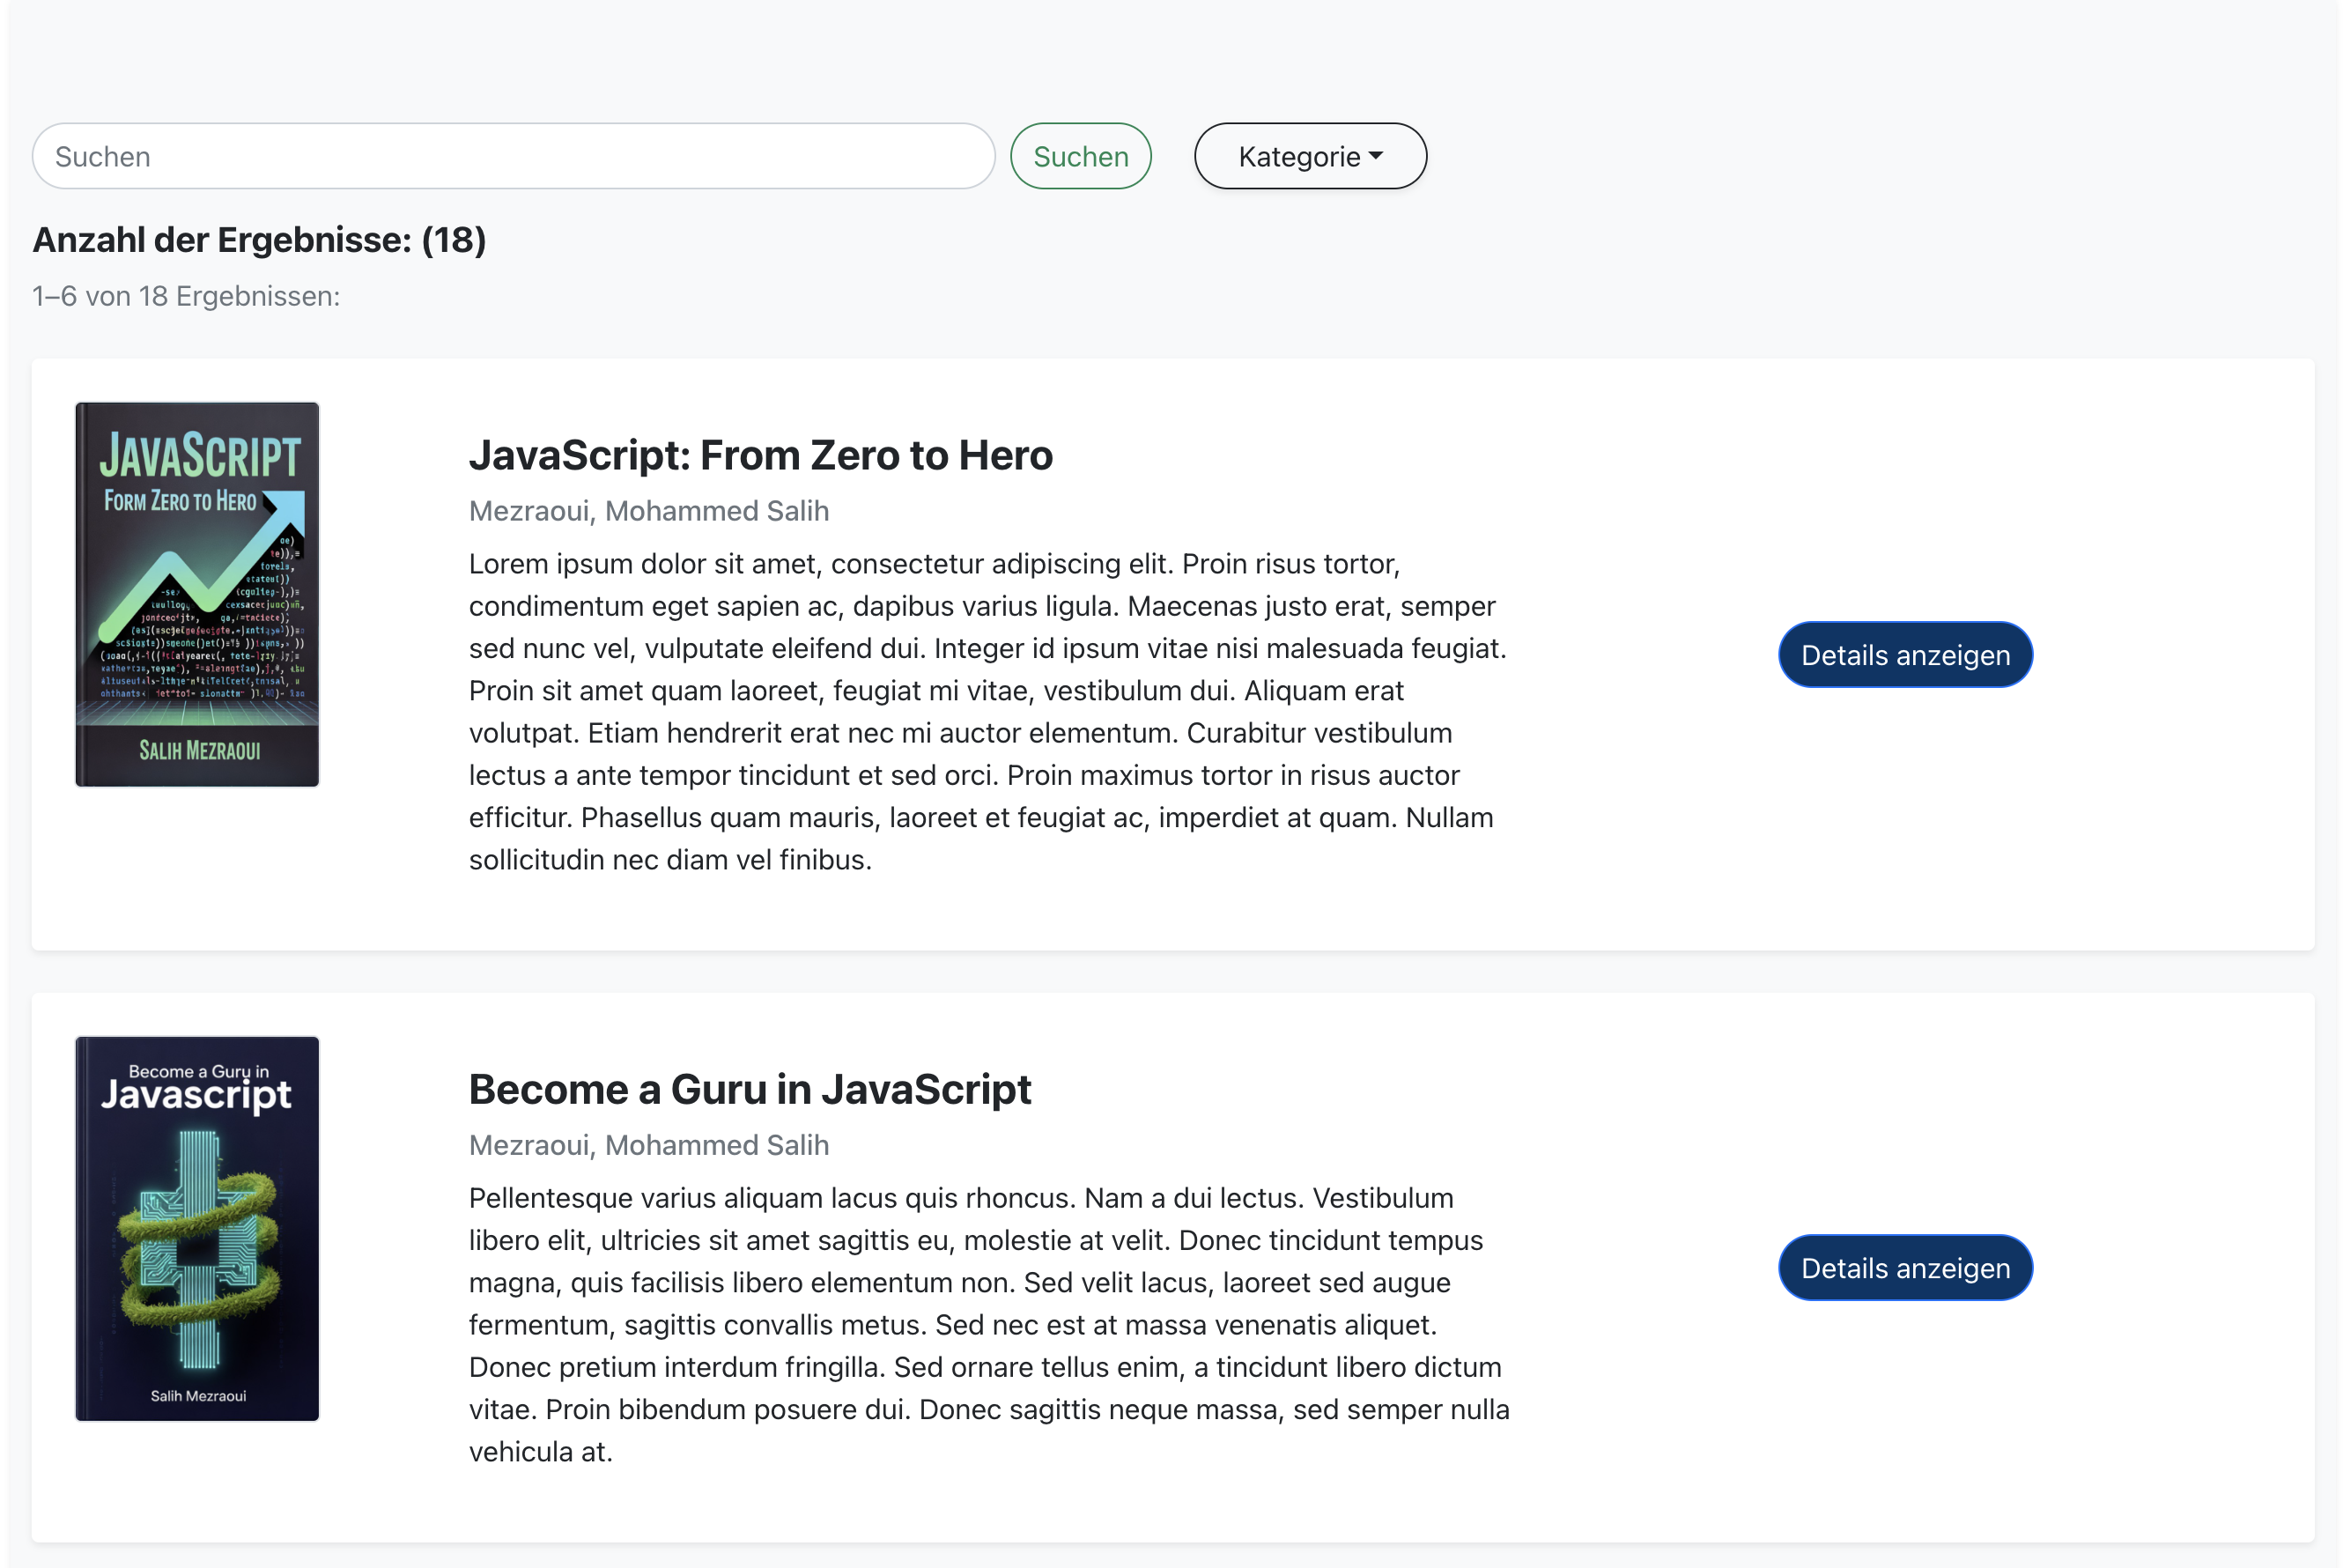
\includegraphics[width=1.0\textwidth]{images/UI-screenshots/Search-page.png}%\subsection{Startseite (Main Page)}
	\caption{Benutzeroberfläche der Suchseite}
	\label{fig:Search-page}
\end{figure}

\subsection{Buchseite}
Die untenstehende Abbildung  \ref{fig:Book-page} zeigt die Benutzeroberfläche der Buchseite. 

\begin{figure}[H]
	\centering
	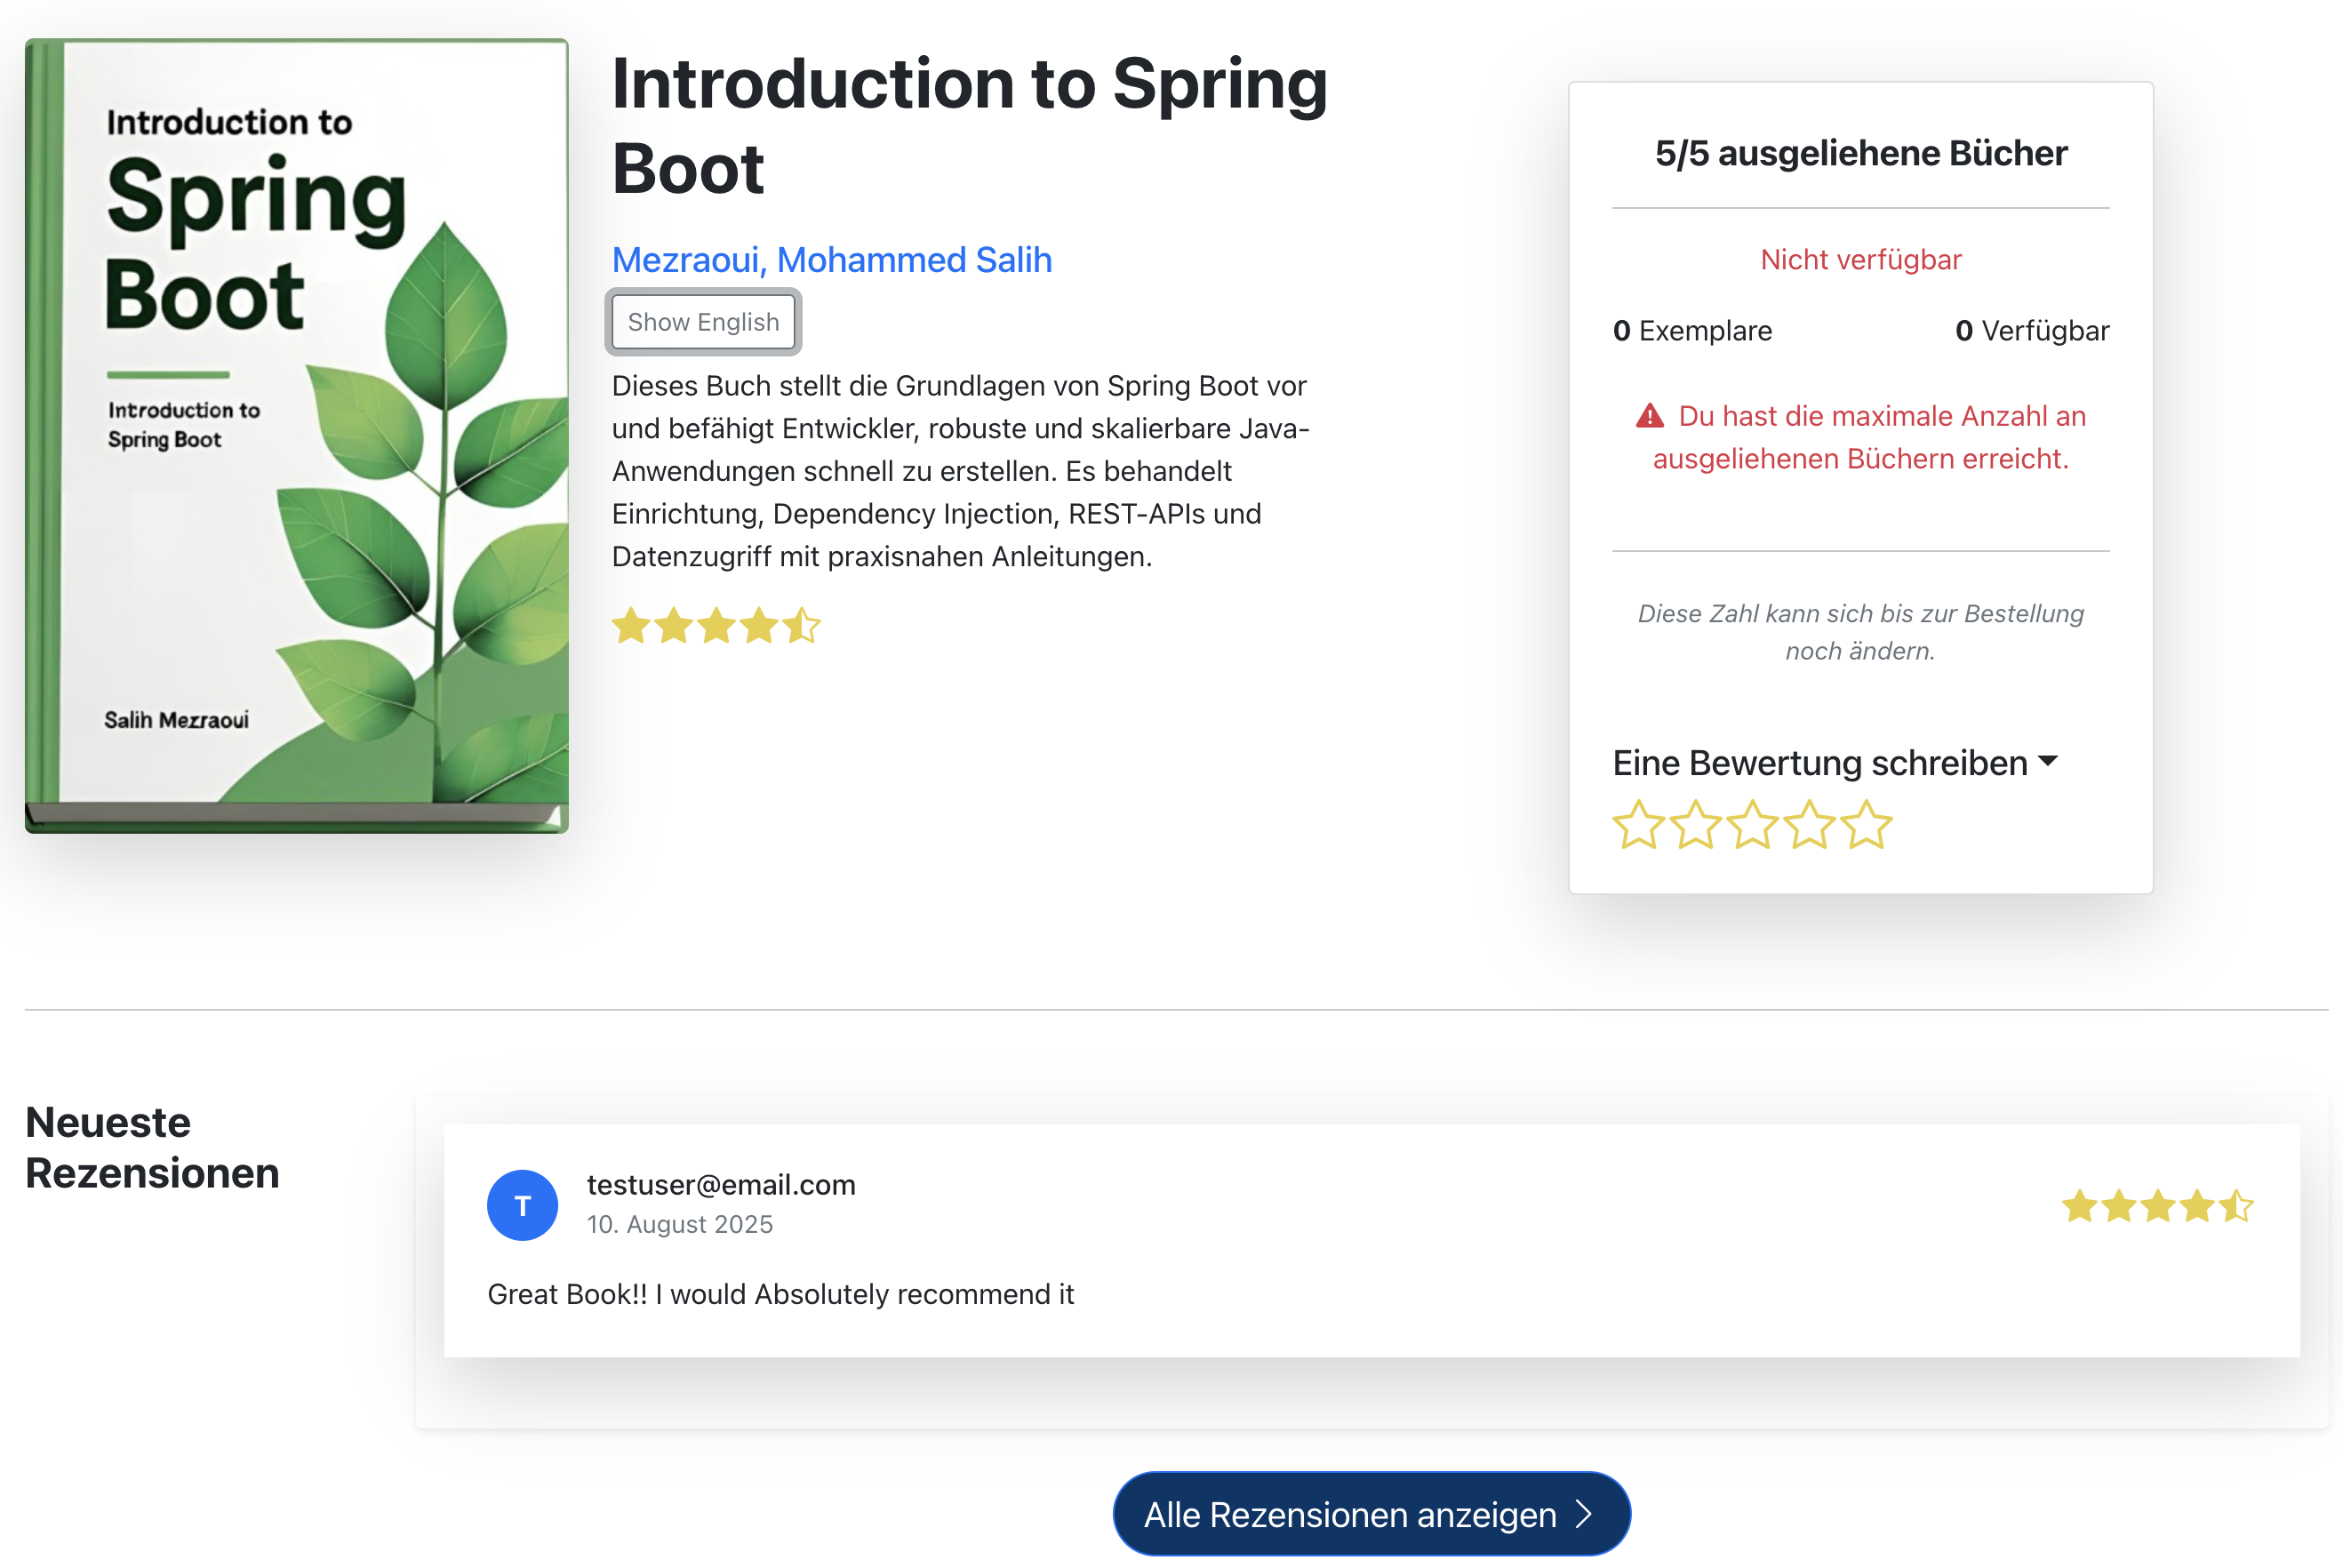
\includegraphics[width=1.0\textwidth]{images/UI-screenshots/Book-Page.png}
	\caption{Benutzeroberfläche der Buchseite}
	\label{fig:Book-page}
\end{figure}

\noindent Die Buchdetailseite stellt umfassende Informationen zu einem einzelnen Buch bereit und enthält folgende Elemente:
\begin{itemize}
	\item Darstellung des Buchcovers.
	\item Anzeige des Buchtitels und des Autors.
	\item Buchbeschreibung mit der Möglichkeit, zwischen deutscher und englischer Sprache zu wechseln, unabhängig von der Spracheinstellung der Gesamtanwendung.
	\item Bewertungssystem zur Anzeige der durchschnittlichen Nutzerbewertung.
	\item Rechte Seitenleiste mit folgenden Informationen:
	\begin{itemize}
		\item Anzahl der vom aktuellen Benutzer ausgeliehenen Exemplare,
		\item Anzahl der derzeit verfügbaren Exemplare,
		\item Gesamtanzahl der im Bestand befindlichen Exemplare.
	\end{itemize}
	\item Übersicht der Nutzerbewertungen zum Buch.
	\item Link zur vollständigen Liste aller Reviews.
\end{itemize}

\section{Bibliotheksaktivität}
In diesem Abschnitt werden die Funktionen zur Verwaltung aktueller und vergangener Ausleihen dargestellt.

\subsection{Ausleihen}
Die untenstehende Abbildung \ref{fig:Loans-Page} zeigt das Design der \texttt{Ausleihen} Seite. 

\begin{figure}[H]
	\centering
	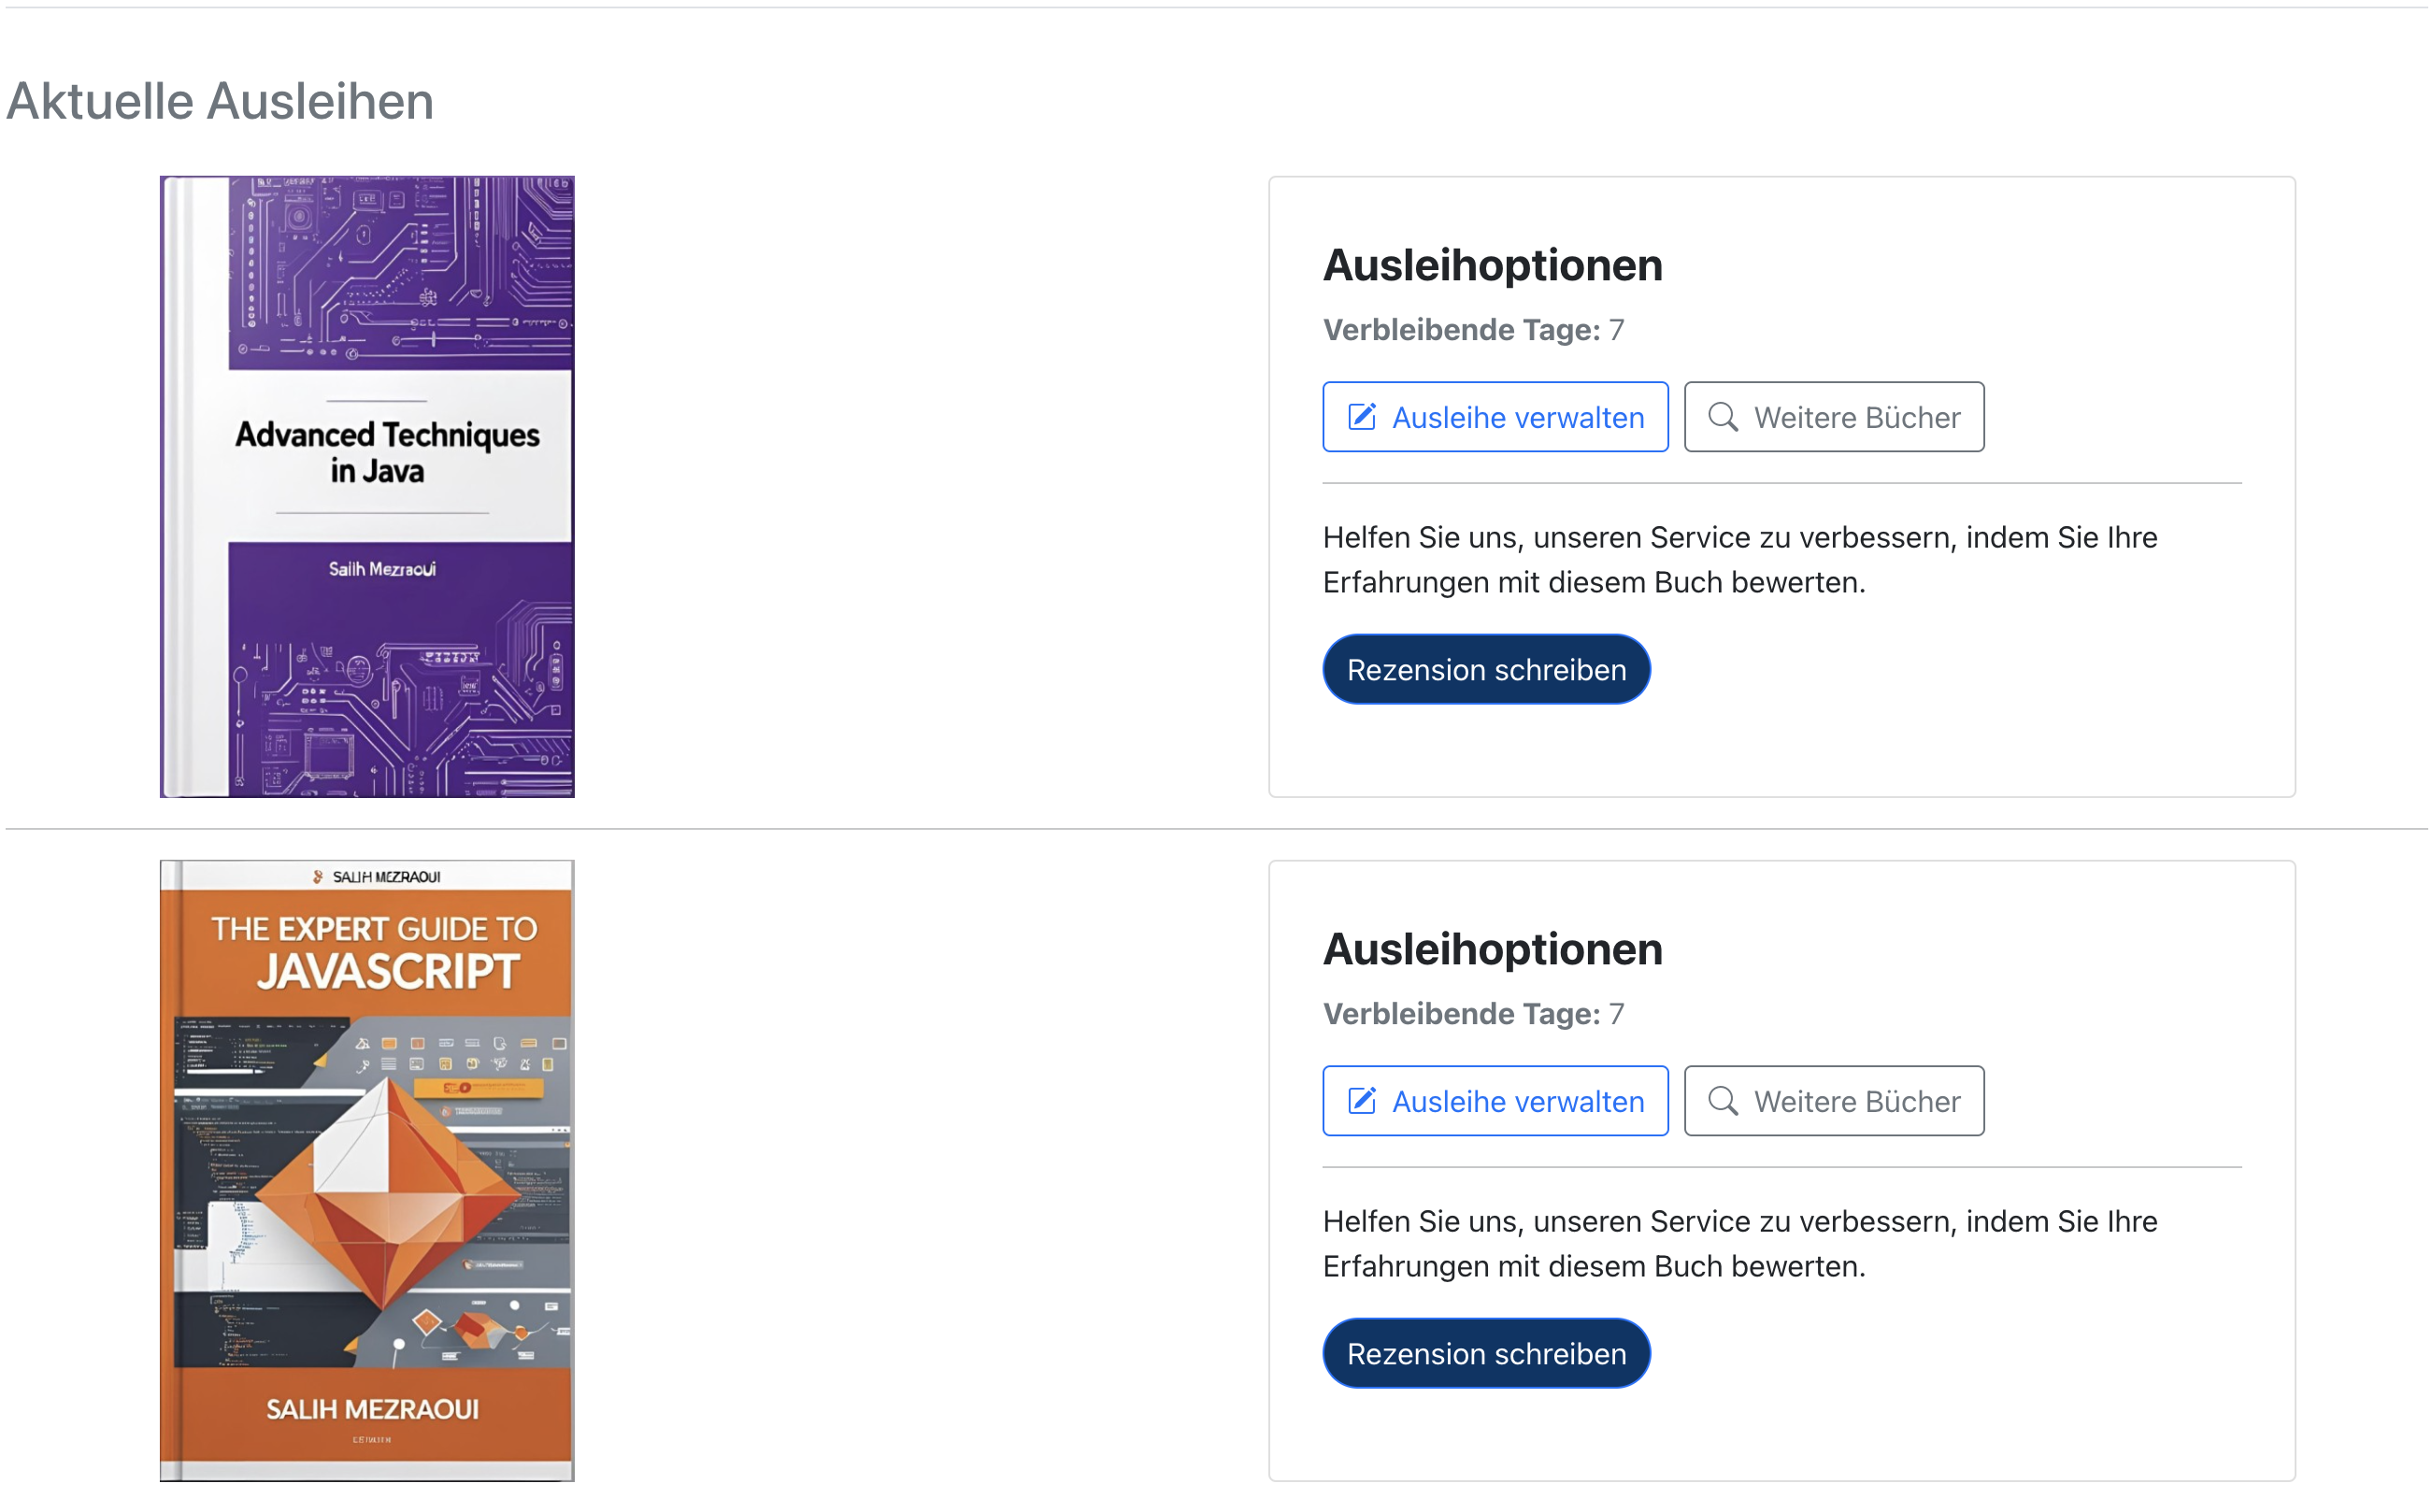
\includegraphics[width=1.0\textwidth]{images/UI-screenshots/Loans-Page.png}
	\caption{Benutzeroberfläche der Ausleihseite}
	\label{fig:Loans-Page}
\end{figure}

Die Ausleiheseite ermöglicht es Nutzerinnen und Nutzern, ihre aktuell ausgeliehenen Bücher zu verwalten. Sie enthält folgende Elemente:

\begin{itemize}
	\item Liste aller aktuell ausgeliehenen Bücher.
	\item Anzeige der verbleibenden Tage bis zur Rückgabe jedes Buches.
	\item Verwaltungsoptionen pro Buch:
	\begin{itemize}
		\item Rückgabe des Buches,
		\item Verlängerung der Leihfrist.
	\end{itemize}
	\item Schaltfläche zur Suche nach weiteren Büchern.
	\item Link zum Verfassen einer Rezension für das jeweilige Buch.
\end{itemize}

\subsection{Ausleihhistorie}
Die untenstehende Abbildung \ref{fig:Loans-History-Page} zeigt das Design der Seite \texttt{Ausleihverlauf}. Diese Seite enthält die Historie der vom Nutzer ausgeliehenen Bücher, einschließlich des Ausleih- und Rückgabedatums.

\begin{figure}[H]
	\centering
	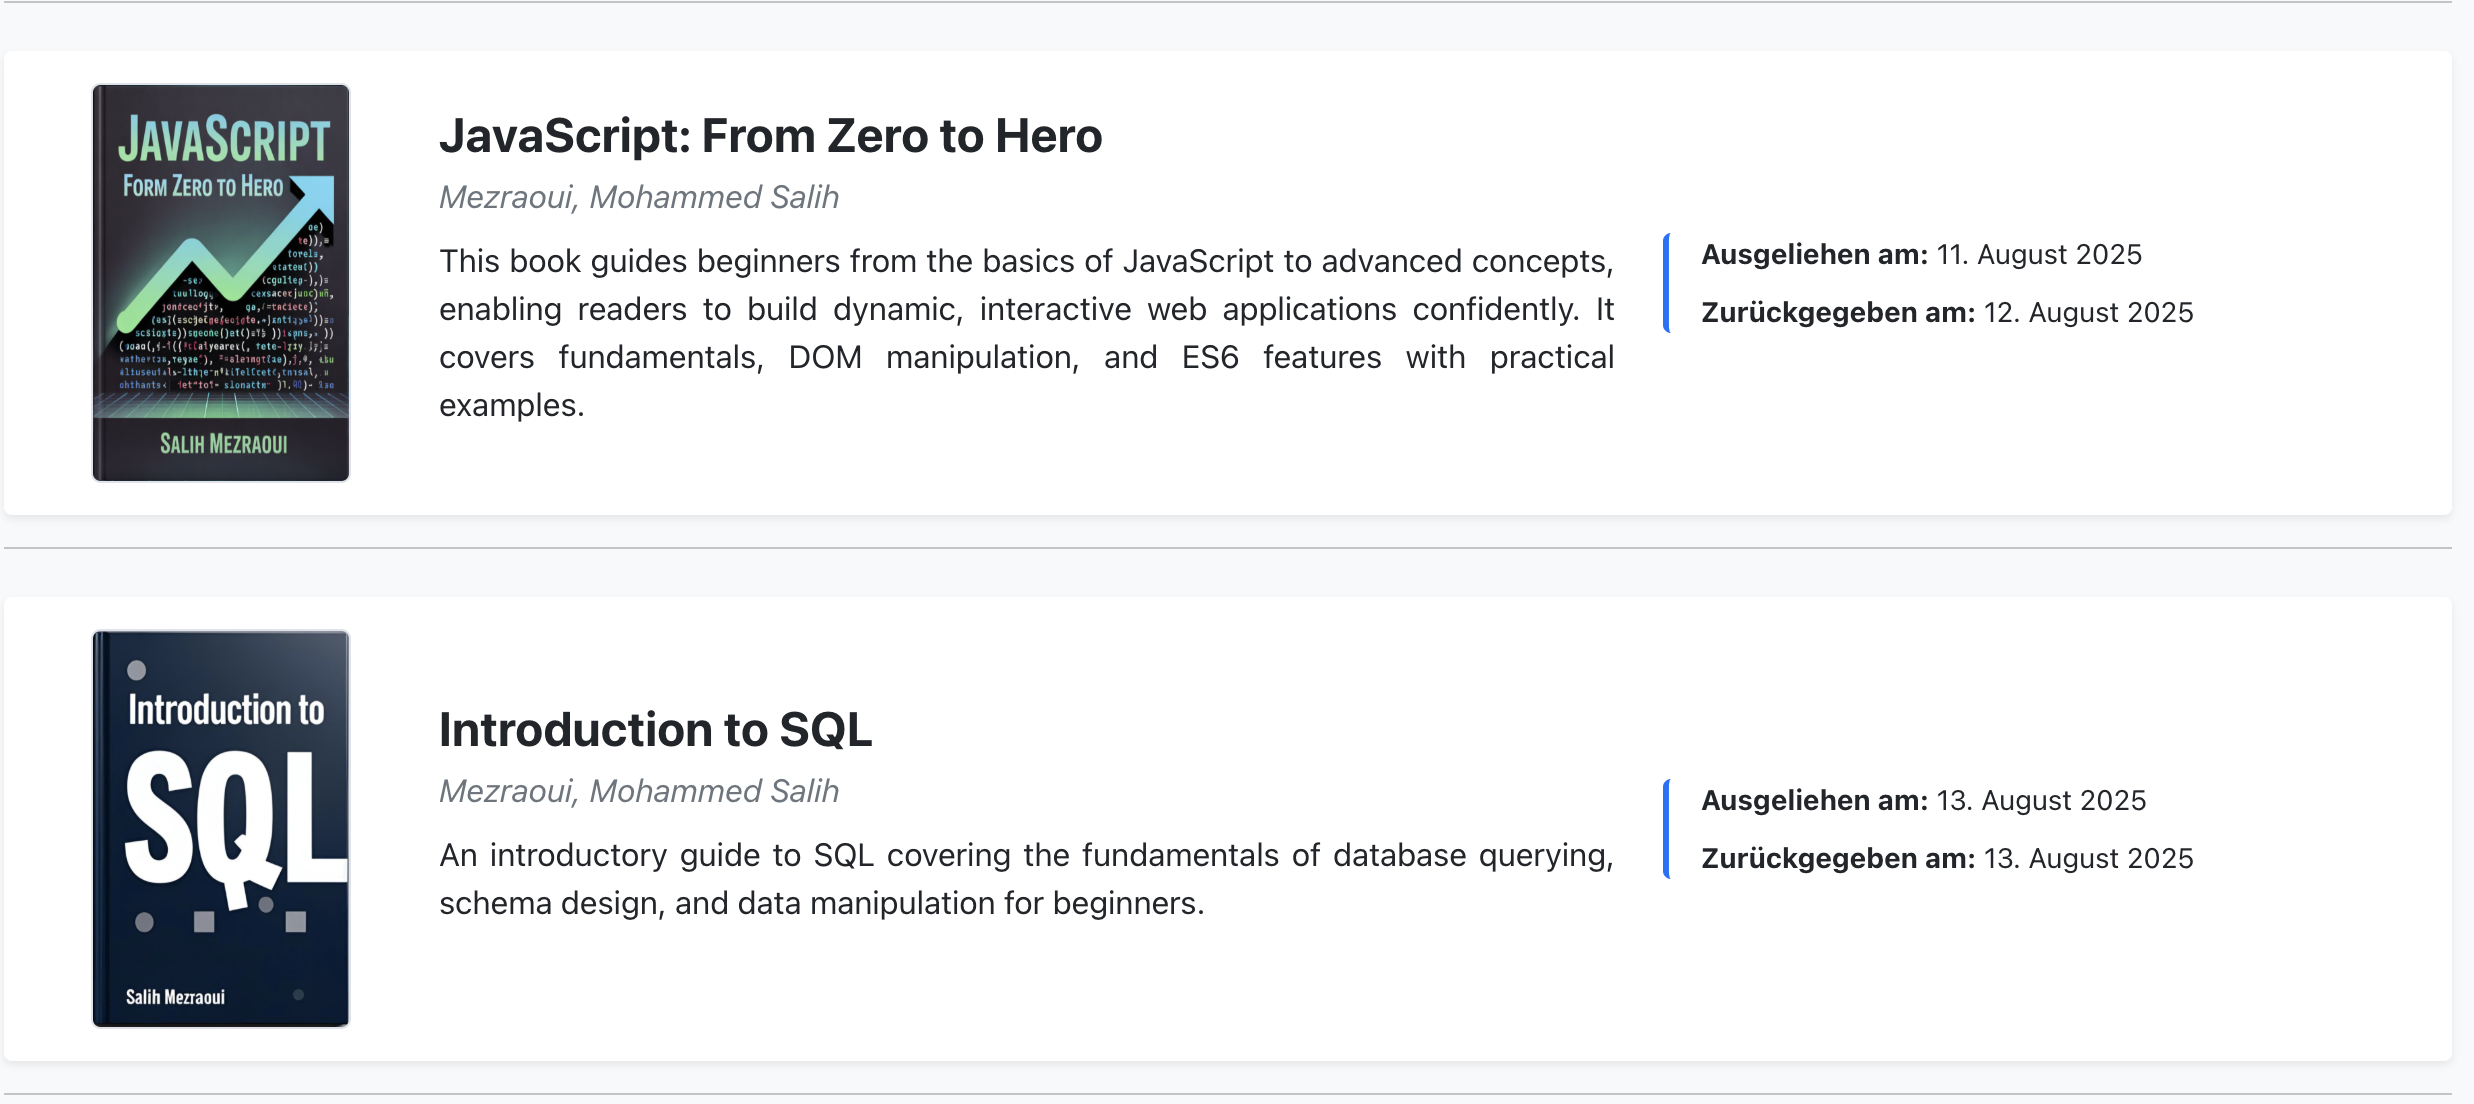
\includegraphics[width=1.0\textwidth]{images/UI-screenshots/Loans-History.png}
	\caption{Benutzeroberfläche der Ausleihverlaufsseite}%\subsection{Bibliotheksservice (Library Service)}
	\label{fig:Loans-History-Page}
\end{figure}

\section{Bibliotheksdienste}
In diesem Abschnitt werden die Bibliotheksdienste vorgestellt, insbesondere die Benutzeroberfläche zur Übermittlung von Anfragen sowie der persönliche Nachrichtenverlauf mit den jeweiligen Antworten.

\noindent Die folgende Abbildung \ref{fig:Message-Send} zeigt die Benutzeroberfläche, über die Benutzer einzelne Anfragen oder Nachrichten an die Administratoren der Bibliothek senden können.

\begin{figure}[H]
	\centering
	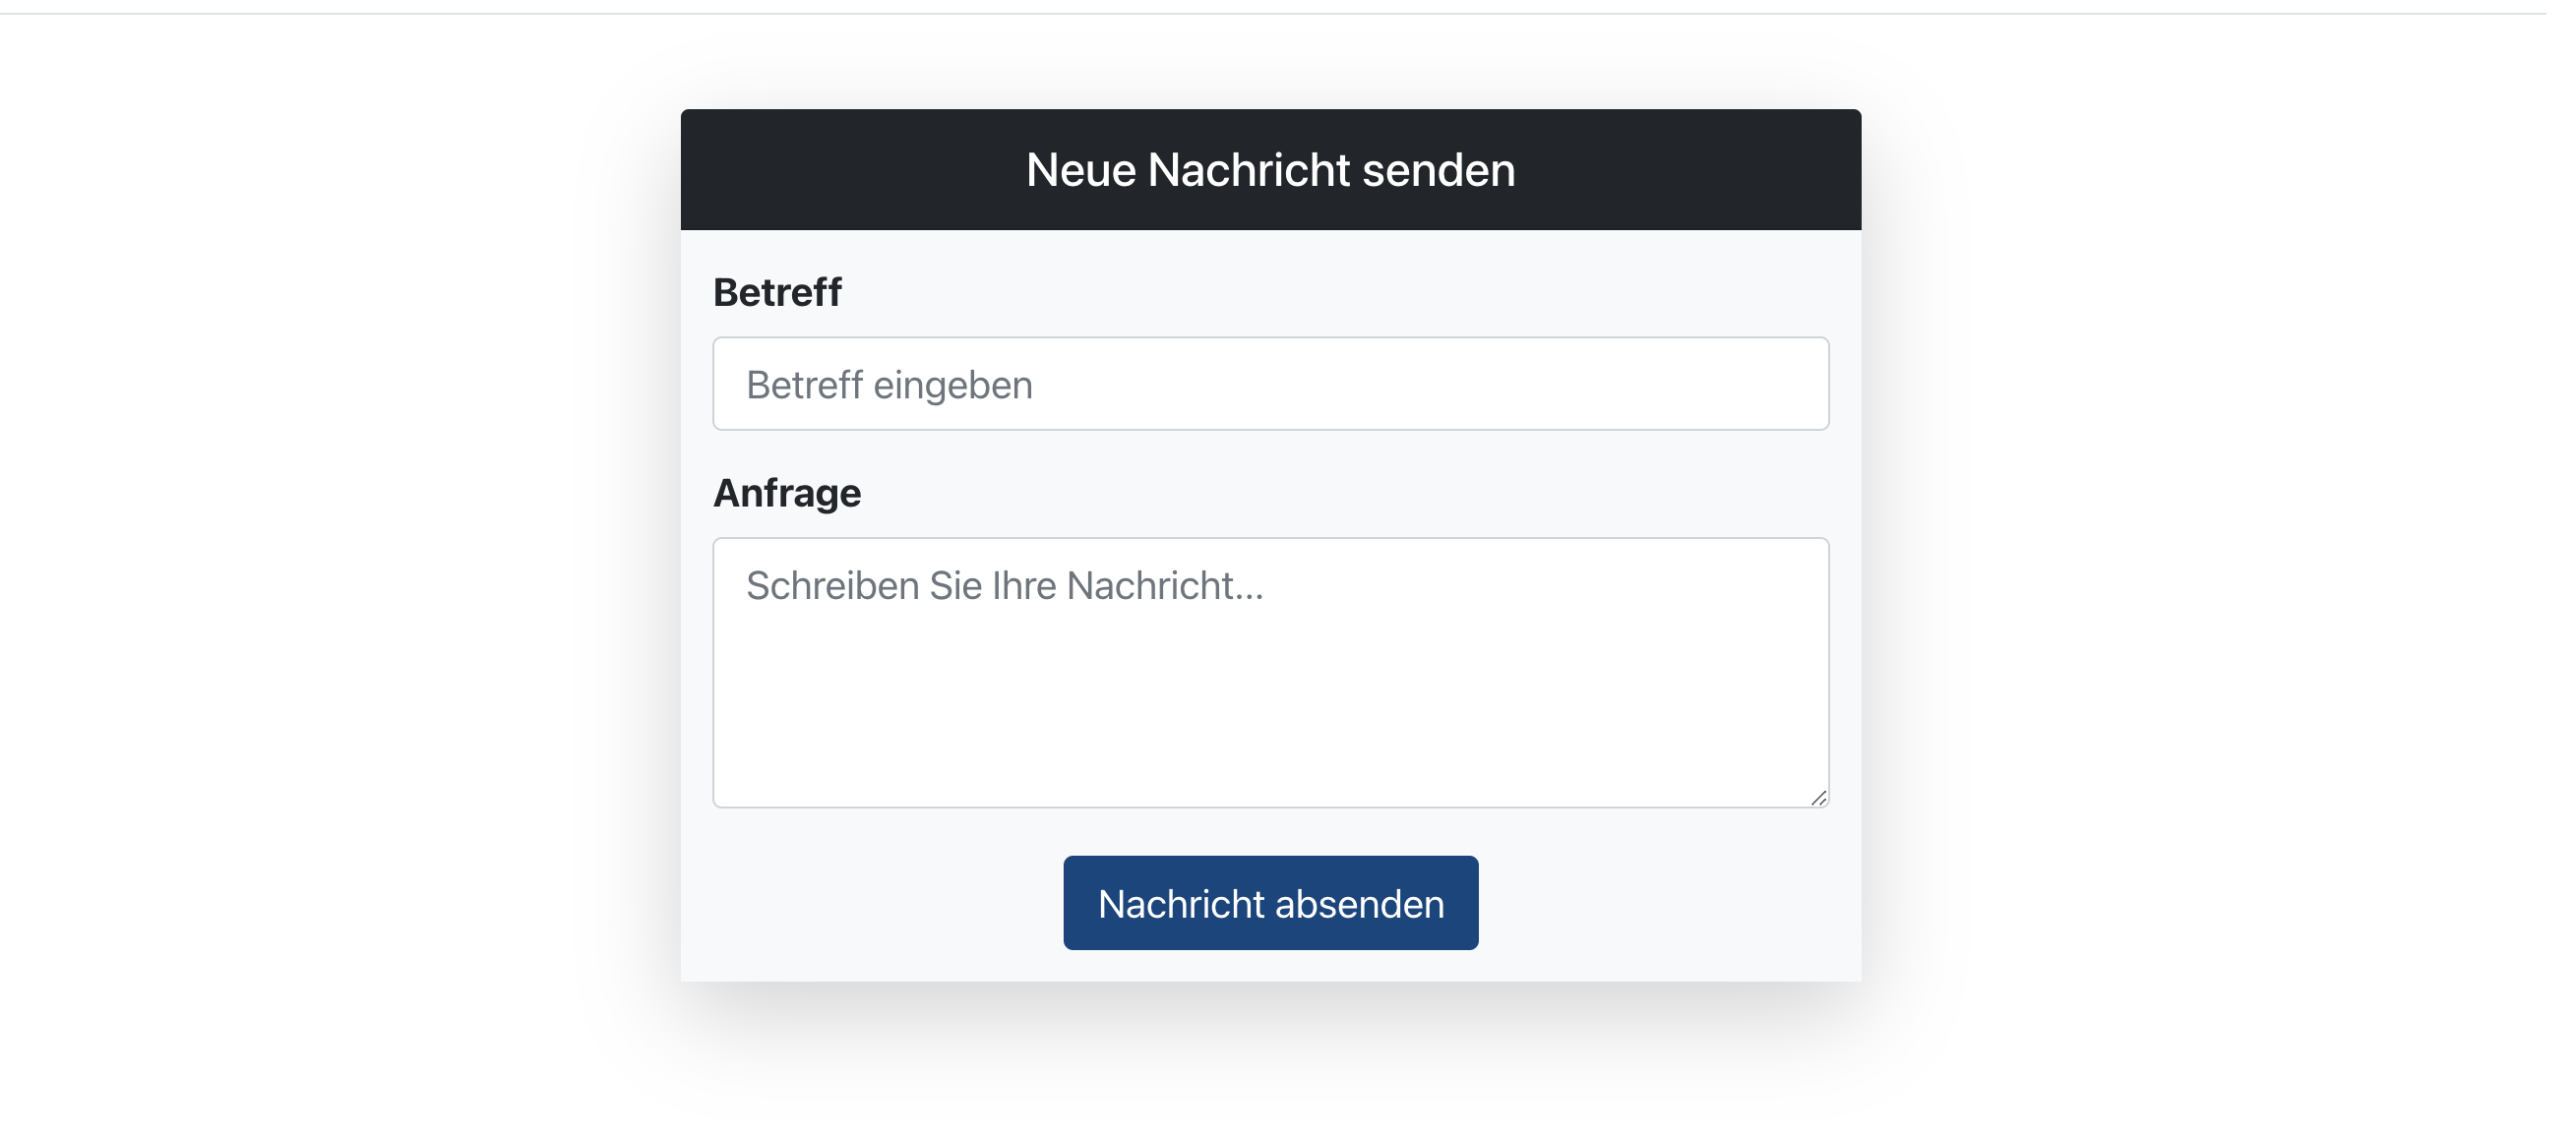
\includegraphics[width=1.0\textwidth]{images/UI-screenshots/Message-Send.png}
	\caption{Benutzeroberfläche zum Versenden von Anfragen}
	\label{fig:Message-Send}
\end{figure}

\noindent Die Abbildung \ref{fig:Messages-History} veranschaulicht den Verlauf sämtlicher ausgetauschter Nachrichten, einschließlich der gestellten Fragen und der dazugehörigen Antworten.

\begin{figure}[H]
	\centering
	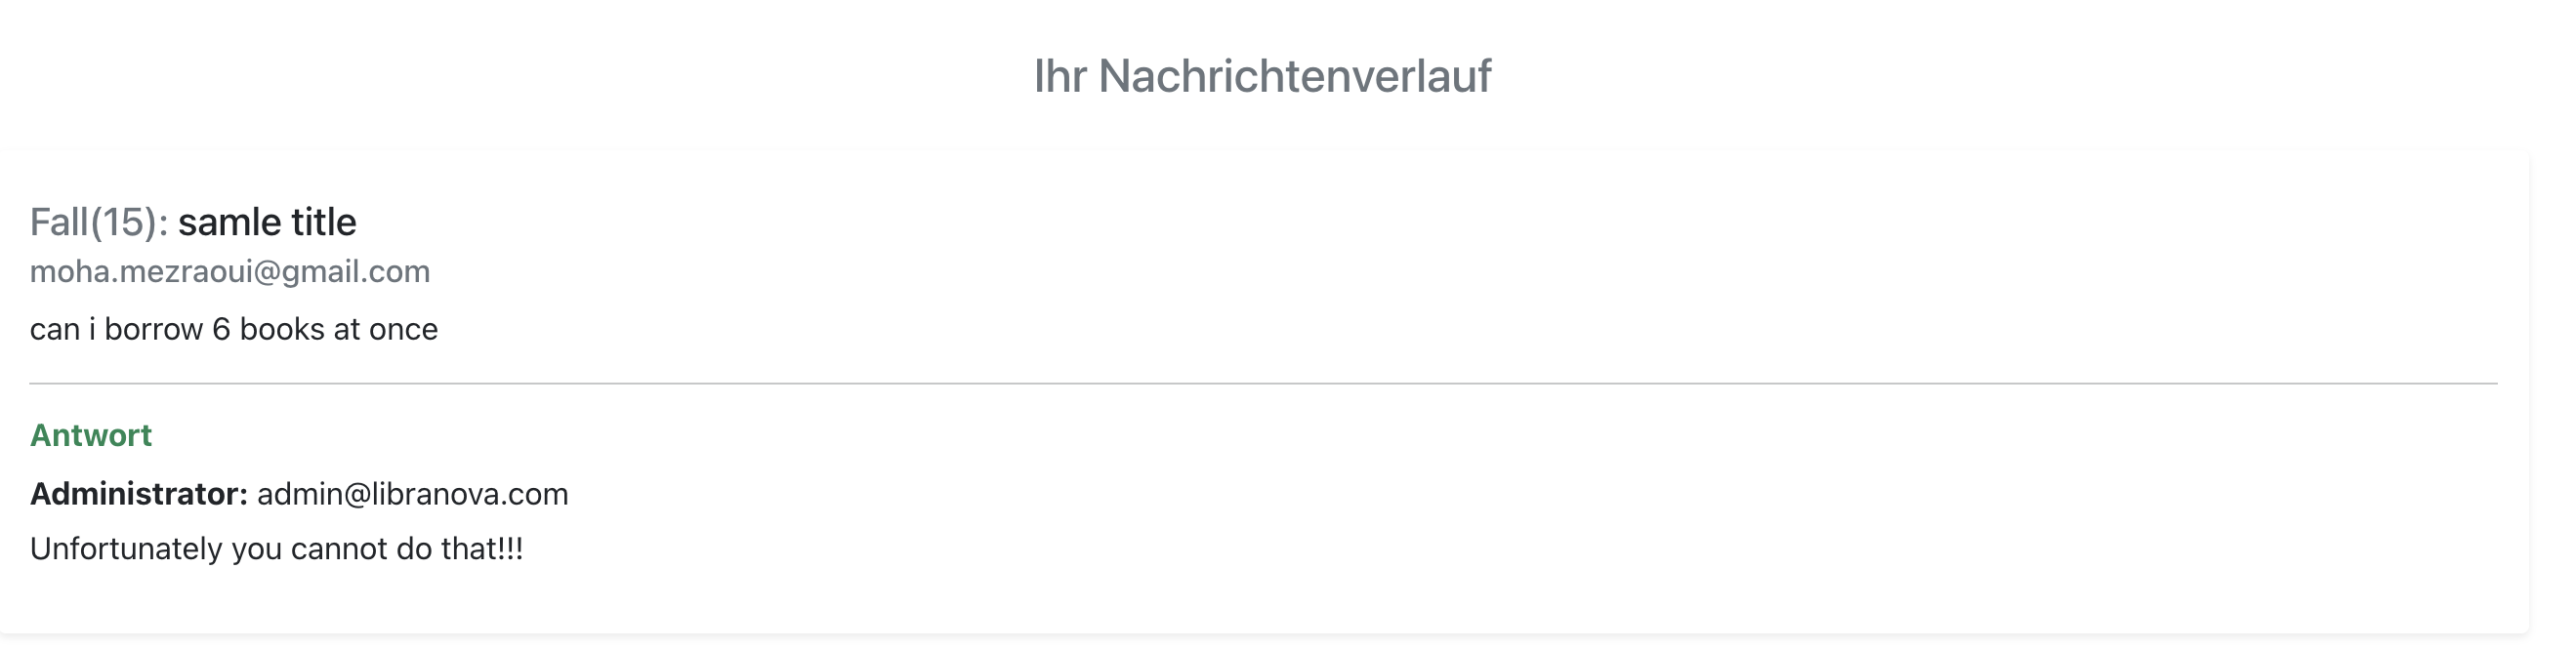
\includegraphics[width=1.0\textwidth]{images/UI-screenshots/Messages-History.png}
	\caption{Nachrichtenverlauf zwischen Nutzer und Bibliothek}
	\label{fig:Messages-History}
\end{figure}

\section{Bezahlungsseite}

In diesem Abschnitt wird die Benutzeroberfläche zur Verwaltung von Zahlungsinformationen und offenen Gebühren vorgestellt. \\

\noindent Abbildung \ref{fig:Outstanding-payment} zeigt das Layout, das angezeigt wird, wenn ein Benutzer ausstehende Zahlungen zu begleichen hat. 

\begin{figure}[H]
	\centering
	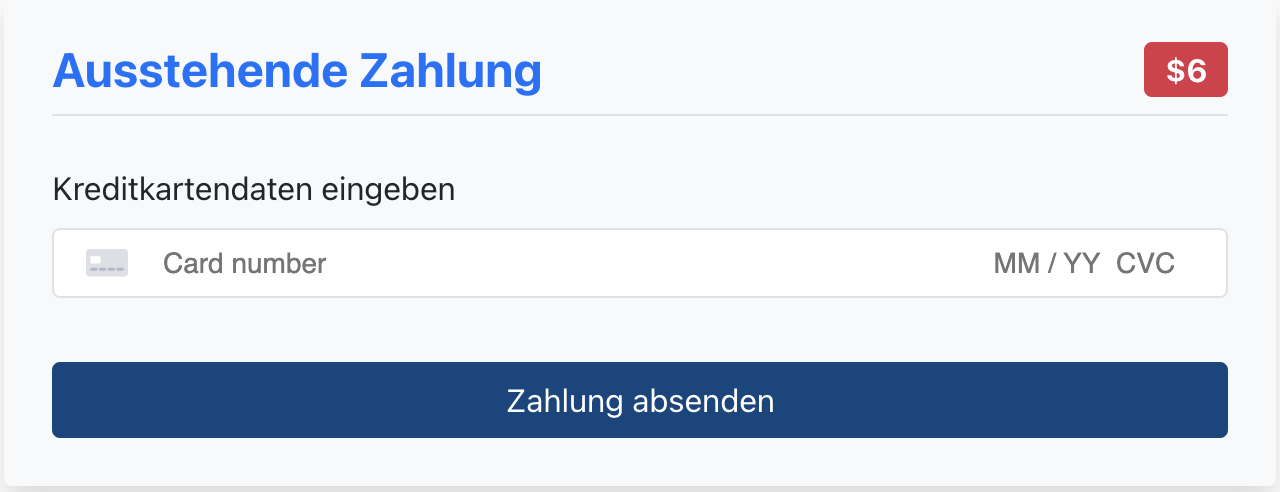
\includegraphics[width=1.0\textwidth]{images/UI-screenshots/Outstanding-payment.png}
	\caption{Benutzeroberfläche bei ausstehenden Zahlungen}
	\label{fig:Outstanding-payment}
\end{figure}

\noindent Wenn keine offenen Gebühren vorliegen, wird dem Nutzer die in Abbildung \ref{fig:No-Payment} dargestellte Ansicht präsentiert. Sie bestätigt, dass derzeit keine Zahlungen erforderlich sind.

\begin{figure}[H]
	\centering
	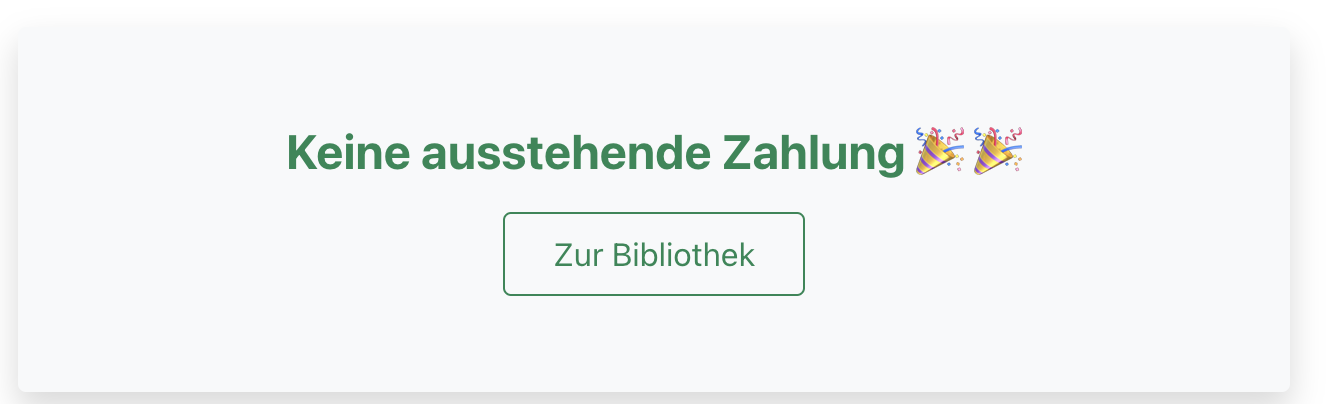
\includegraphics[width=1.0\textwidth]{images/UI-screenshots/No-Payment.png}
	\caption{Benutzeroberfläche bei keinen offenen Zahlungen}
	\label{fig:No-Payment}
\end{figure}

\section{Admin-Bereich}

Der Admin-Bereich bietet eine dedizierte Oberfläche zur Verwaltung der Bibliotheksressourcen und zur Interaktion mit Benutzeranfragen. In diesem Abschnitt werden die Verwaltungsfunktionen dargestellt, die einem Administrator zur Verfügung stehen.

\subsection{Neues Buch hinzufügen}
\noindent Die erste Funktion (siehe \ref{fig:Add-New-Book})ermöglicht es dem Administrator, neue Bücher in das System aufzunehmen. Hierzu gibt er relevante Informationen wie Titel, Autor, Kategorie, eine kurze Beschreibung sowie die Anzahl der verfügbaren Exemplare an. Zusätzlich kann ein Bild des Buchcovers hochgeladen werden. Nach dem Ausfüllen der Felder wird durch Klicken auf die Schaltfläche \textit{"Buch hinzufügen"} ein neuer Eintrag erstellt.
\begin{figure}[H]
	\centering
	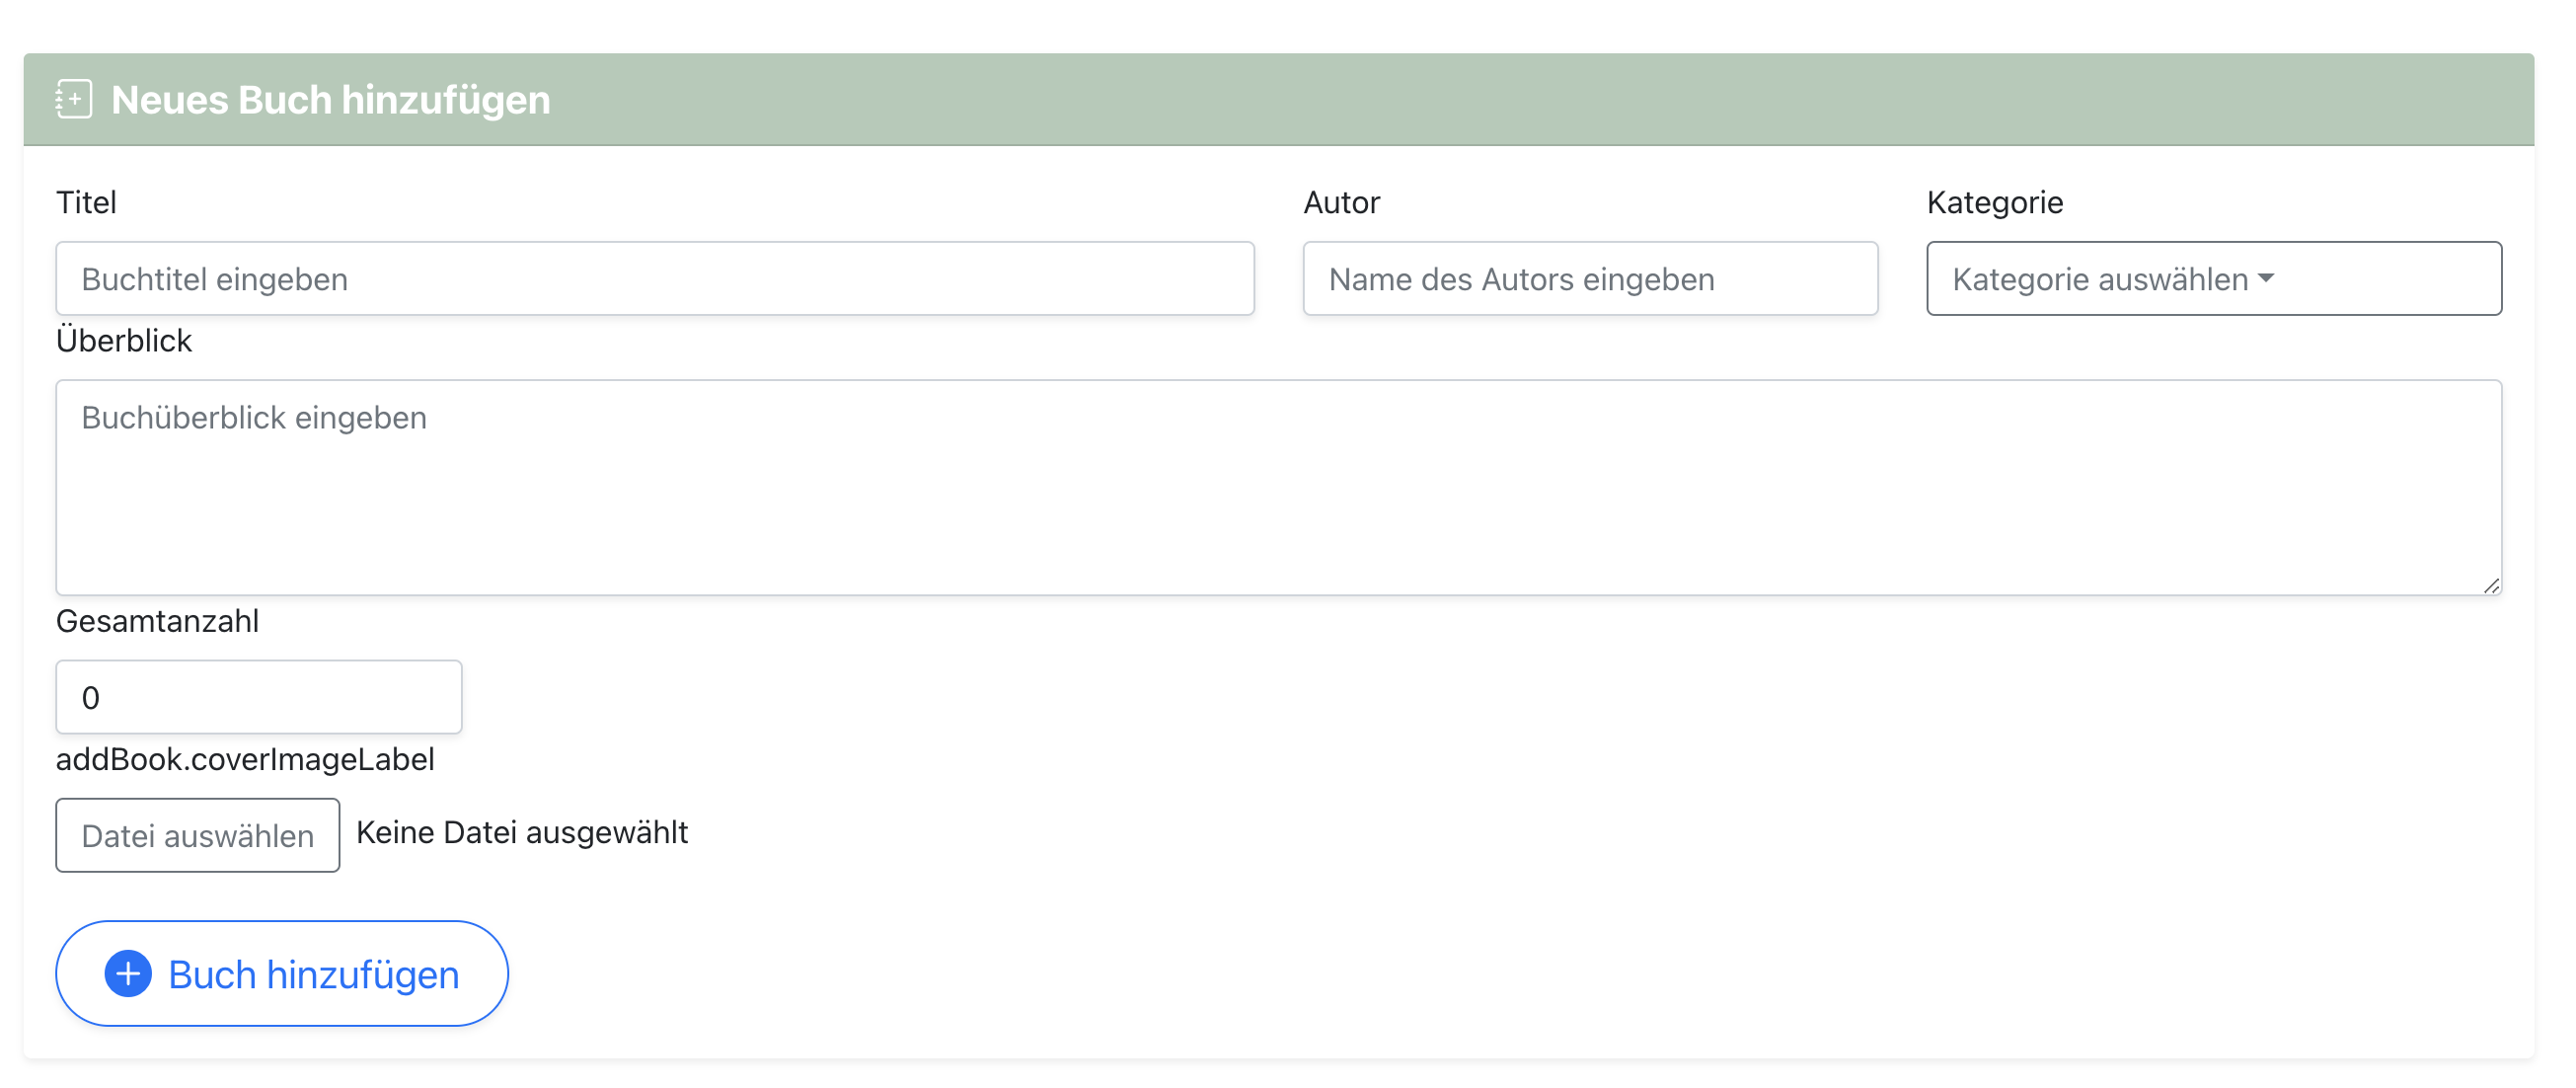
\includegraphics[width=1.0\textwidth]{images/UI-screenshots/Add-New-Book.png}
	\caption{Benutzeroberfläche bei keinen offenen Zahlungen}
	\label{fig:Add-New-Book}
\end{figure}

\subsection{Bücher verwalten}

\noindent Der Administrator kann bestehende Bücher verwalten, indem er die Anzahl der verfügbaren Exemplare anpasst oder Bücher vollständig aus dem System entfernt. Die folgende Abbildung \ref{fig:Manage-Books} zeigt die Verwaltungsoberfläche, über die solche Änderungen vorgenommen werden können.

\begin{figure}[H]
	\centering
	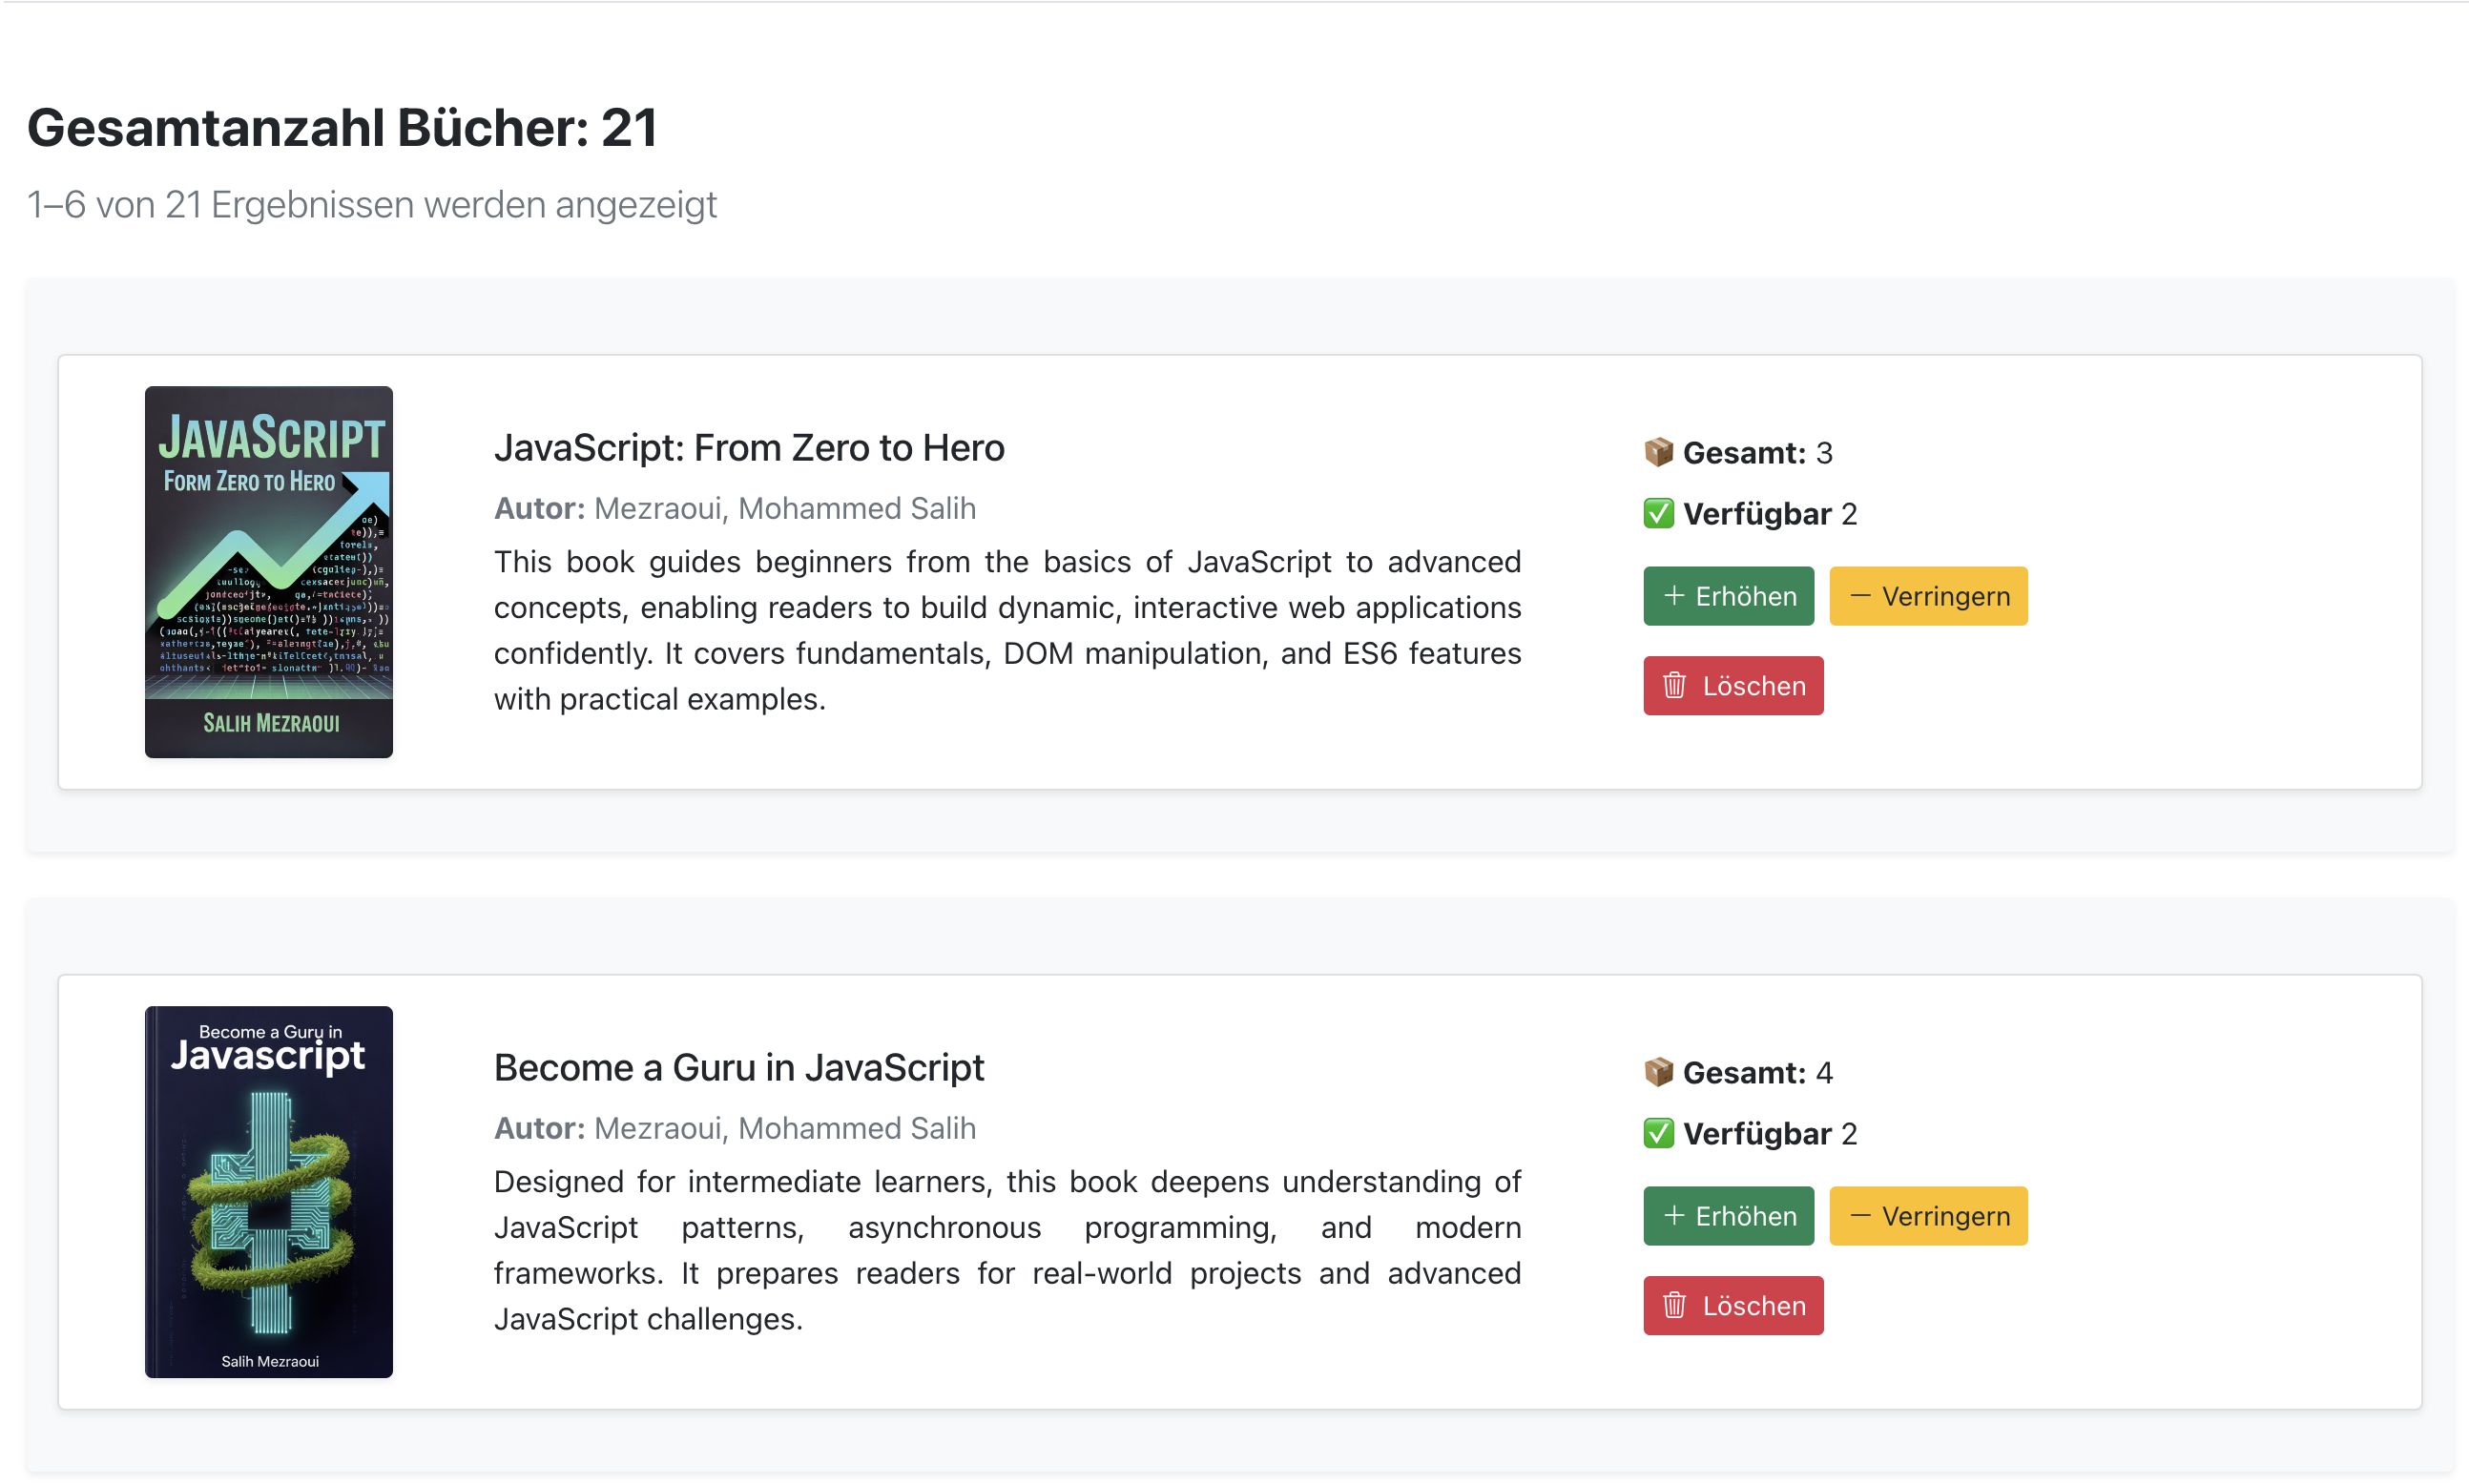
\includegraphics[width=1.0\textwidth]{images/UI-screenshots/Manage-Books.png}
	\caption{Benutzeroberfläche bei keinen offenen Zahlungen}
	\label{fig:Manage-Books}
\end{figure}
\subsection{Nachrichten}

\noindent In diesem Bereich kann der Administrator auf Anfragen von Benutzern antworten. Die Benutzerfrage wird angezeigt und kann direkt über das vorgesehene Textfeld beantwortet werden. Eine Schaltfläche ermöglicht das Senden der Antwort. Die Abbildung \ref{fig:Messages-Responses} zeigt die zugehörige Benutzeroberfläche.

\begin{figure}[H]
	\centering
	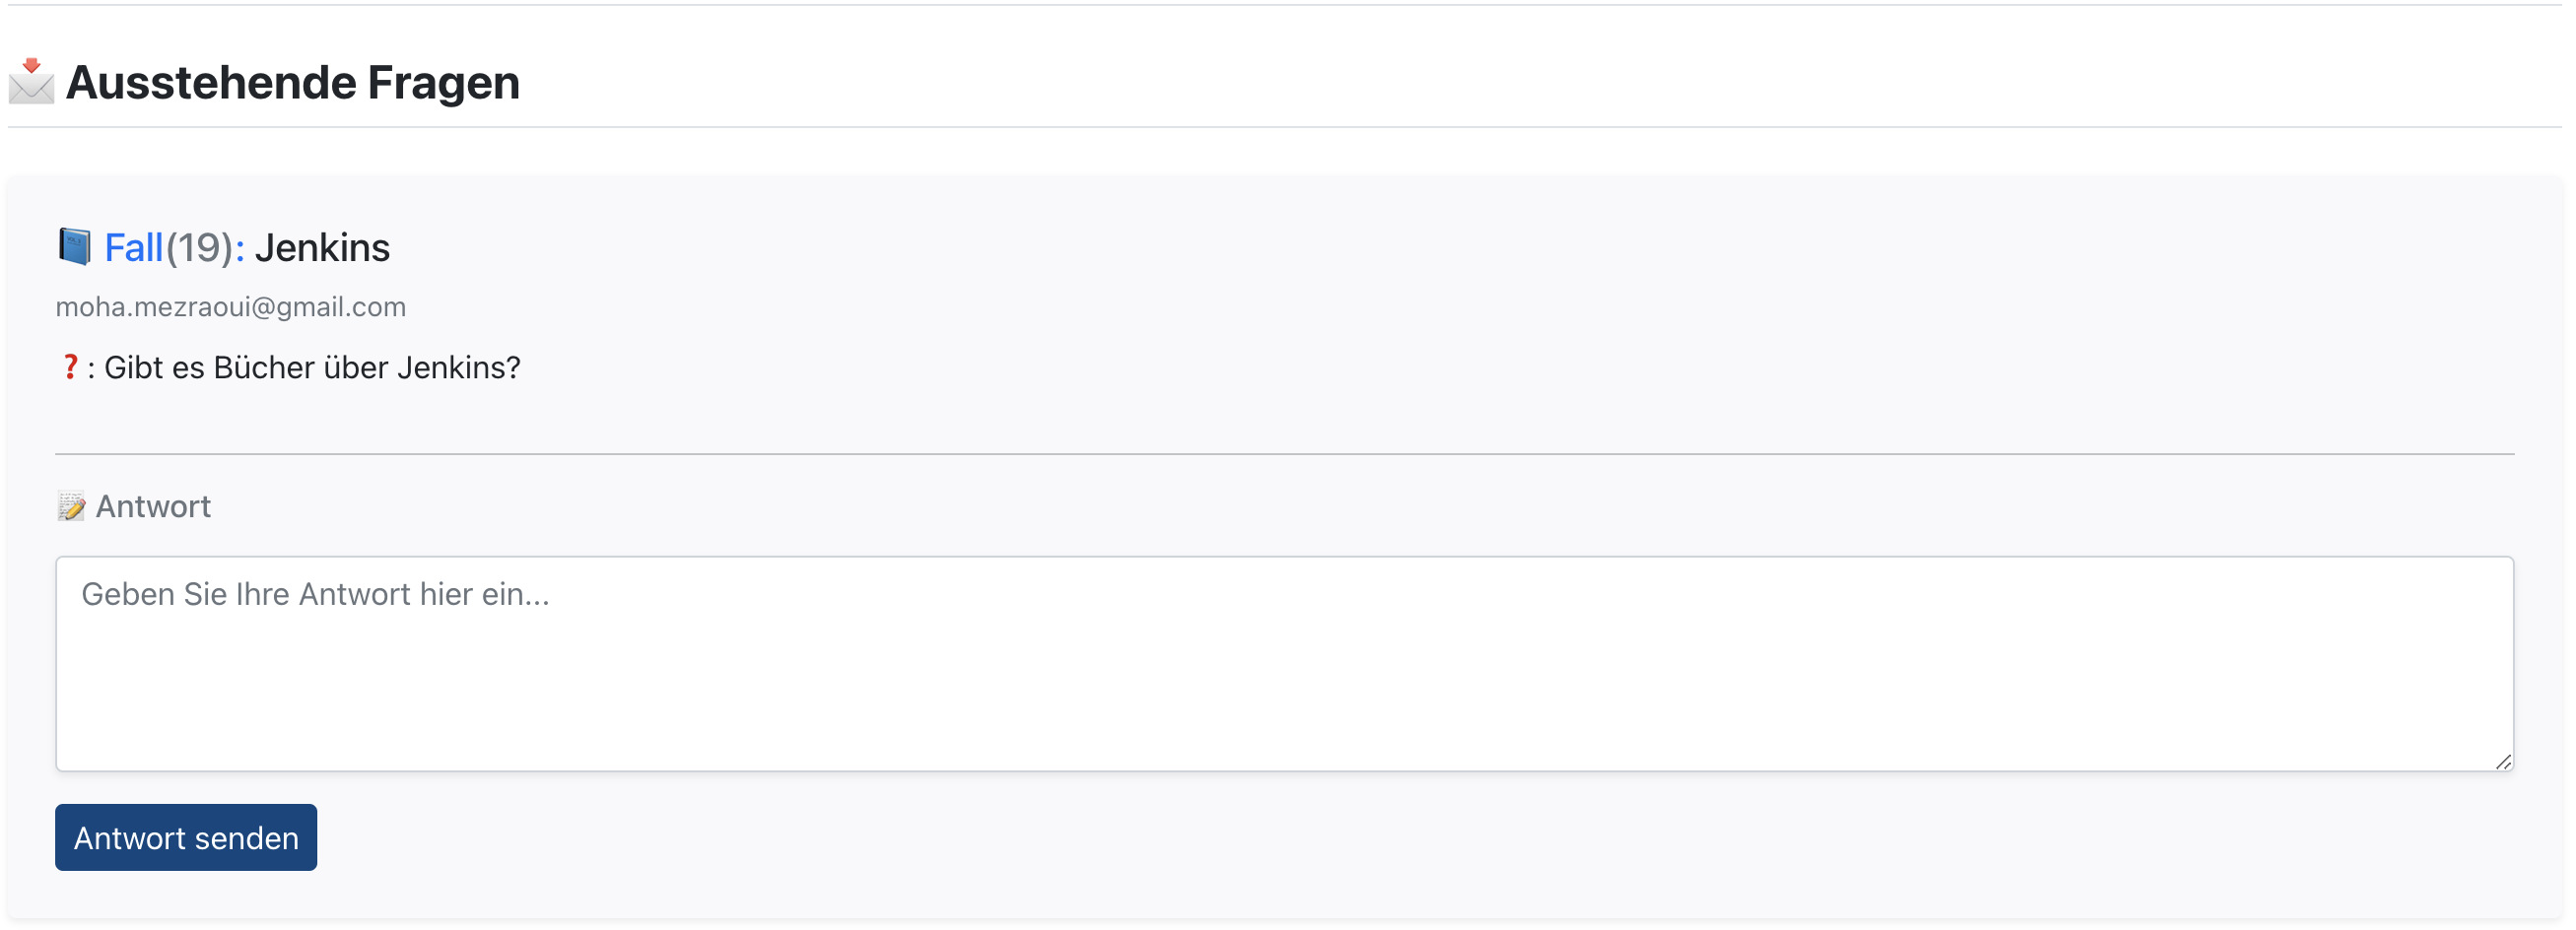
\includegraphics[width=1.0\textwidth]{images/UI-screenshots/Messages-Responses.png}
	\caption{Benutzeroberfläche bei keinen offenen Zahlungen}
	\label{fig:Messages-Responses}
\end{figure}




















